%-----------------------------------------------------------------
%	BASIC DOCUMENT LAYOUT
%-----------------------------------------------------------------
\documentclass[paper=a4, fontsize=12pt, twoside=semi]{scrartcl}
\usepackage[T1]{fontenc}
\usepackage[utf8]{inputenc}
\usepackage{lmodern}
\usepackage{slantsc}
\usepackage{microtype}
\usepackage[british]{babel}

% Bibliography
\usepackage[backend=bibtex, style=trad-abbrv, sorting=none, maxbibnames=5]{biblatex}
\addbibresource{bibliography.bib}
\makeatletter
	\def\blx@maxline{77}
\makeatother

% Sectioning layout
\addtokomafont{sectioning}{\normalfont\scshape}
\usepackage{tocstyle}
\usetocstyle{standard}
\renewcommand*\descriptionlabel[1]{\hspace\labelsep\normalfont\bfseries{#1}}

% Empty pages
\usepackage{etoolbox}
% \pretocmd{\toc}{\cleardoubleevenemptypage}{}{}
\pretocmd{\section}{\cleardoubleevenemptypage}{}{}
\pretocmd{\part}{\cleardoubleevenemptypage\thispagestyle{empty}}{}{}
\renewcommand\partheadstartvskip{\clearpage\null\vfil}
\renewcommand\partheadmidvskip{\par\nobreak\vskip 20pt\thispagestyle{empty}}

% Paragraph indentation behaviour
\setlength{\parindent}{0pt}
\setlength{\parskip}{0.3\baselineskip plus2pt minus2pt}
\newcommand{\sk}{\medskip\noindent}

% Fancy header and footer
\usepackage{fancyhdr}
\pagestyle{fancyplain}
\fancyhead[LO]{\thepage}
\fancyhead[CO]{}
\fancyhead[RO]{\nouppercase{\mytitle}}
\fancyhead[LE]{\nouppercase{\leftmark}}
\fancyhead[CE]{}
\fancyhead[RE]{\thepage}
\fancyfoot{}
\renewcommand{\headrulewidth}{0.3pt}
\renewcommand{\footrulewidth}{0pt}
\setlength{\headheight}{13.6pt}

%-----------------------------------------------------------------
%	MATHS AND SCIENCE
%-----------------------------------------------------------------
\usepackage{amsmath,amsfonts,amsthm,amssymb}
\usepackage{xfrac}
\usepackage[a]{esvect}
\usepackage{chemformula}
\usepackage{graphicx}

\usepackage[arrowdel]{physics}
	\renewcommand{\vnabla}{\vec{\nabla}}
	% \renewcommand{\vectorbold}[1]{\boldsymbol{#1}}
	% \renewcommand{\vectorarrow}[1]{\vec{\boldsymbol{#1}}}
	% \renewcommand{\vectorunit}[1]{\hat{\boldsymbol{#1}}}
	\renewcommand{\vectorarrow}[1]{\vec{#1}}
	\renewcommand{\vectorunit}[1]{\hat{#1}}
	\renewcommand*{\grad}[1]{\vnabla #1}
	\renewcommand*{\div}[1]{\vnabla \vdot \va{#1}}
	\renewcommand*{\curl}[1]{\vnabla \cp \va{#1}}
	\let\rot\curl

% SI units
\usepackage[separate-uncertainty=true]{siunitx}
\sisetup{range-phrase = \text{--}, range-units = brackets}
\DeclareSIPrePower\quartic{4}
	%\DeclareSIUnit\micron{\micro\metre}

% Smaller trig functions
\newcommand{\Sin}{\trigbraces{\operatorname{s}}}
\newcommand{\Cos}{\trigbraces{\operatorname{c}}}
\newcommand{\Tan}{\trigbraces{\operatorname{t}}}

% Operator-style notation for matrices
\newcommand*{\mat}[1]{\hat{#1}}

% Matrices in (A|B) form via [c|c] option
\makeatletter
\renewcommand*\env@matrix[1][*\c@MaxMatrixCols c]{%
  \hskip -\arraycolsep
  \let\@ifnextchar\new@ifnextchar
  \array{#1}}
\makeatother

% Shorter \mathcal and \mathbb
\newcommand*{\mc}[1]{\mathcal{#1}}
\newcommand*{\mbb}[1]{\mathbb{#1}}

% Shorter ^\ast and ^\dagger
\newcommand*{\sast}{^{\star}{}}
\newcommand*{\sdag}{^{\dagger}{}}

% Complex and Hermitian conjugates
\newcommand*{\cc}{\,\text{c.c.}}
\newcommand*{\Hc}{\,\text{H.c.}}

% Blackboard bold identity
\usepackage{bbm}
\newcommand*{\bbid}{\mathbbm{1}}

% Shorter displaystyle
\newcommand*{\dsp}{\displaystyle}

% Arrows with text and cancels for developments
\newcommand{\tikzmark}[1]{\tikz[overlay,remember picture] \node (#1) {};}
\tikzset{square arrow/.style={to path={-- ++(0,-.25) -| (\tikztotarget)}}}
\usepackage{cancel}

% Short longitudinal and transverse fields
\newcommand*{\vare}[1]{\va{\mathcal{#1}}}
\newcommand*{\lng}[1]{{#1}_{\parallel}}
\newcommand*{\trn}[1]{{#1}_{\perp}}

% Named equation
\usepackage{stackengine}
\def\stackalignment{r}
\def\useanchorwidth{T}
\def\stacktype{L}
\newlength\eqshift
\setlength\eqshift{\widthof{)}}
\renewcommand\theequation{\thesection.\arabic{equation}}
\let\savetheequation\theequation
\newenvironment{nequation}[1]{%
	\def\thecurrentname{#1}%
	\let\theequation\savetheequation%
	\begin{equation}%
	\renewcommand\theequation{%
		\stackunder{\savetheequation}%
		{{\small\thecurrentname}\hspace{-\the\eqshift}}}%
}{%
	\end{equation}%
	\let\theequation\savetheequation%
	\ignorespacesafterend%
}

%-----------------------------------------------------------------
%	OTHER PACKAGES
%-----------------------------------------------------------------
\usepackage{environ}

% Plots and graphics
\usepackage{pgfplots}
\usepackage{tikz}
	\usetikzlibrary{calc}
\usepackage{color}
	\makeatletter
		\color{black}
		\let\default@color\current@color
	\makeatother

% Richer enumerate, figure, and table support
\usepackage{enumerate}
\usepackage[shortlabels]{enumitem}
\usepackage{float}
\usepackage{tabularx}
\usepackage{booktabs}
	%\setlength{\intextsep}{8pt}
\numberwithin{equation}{section}
\numberwithin{figure}{section}
\numberwithin{table}{section}

% No indentation after certain environments
\makeatletter
\newcommand*\NoIndentAfterEnv[1]{%
	\AfterEndEnvironment{#1}{\par\@afterindentfalse\@afterheading}}
\makeatother
%\NoIndentAfterEnv{thm}
\NoIndentAfterEnv{defi}
\NoIndentAfterEnv{example}
\NoIndentAfterEnv{table}

% Misc packages
\usepackage{ccicons}
\usepackage{lipsum}

%-----------------------------------------------------------------
%	THEOREMS
%-----------------------------------------------------------------
\usepackage{thmtools}

% Theroems layout
\declaretheoremstyle[
	spaceabove=6pt, spacebelow=6pt,
	headfont=\normalfont,
	notefont=\mdseries, notebraces={(}{)},
	bodyfont=\small,
	postheadspace=1em,
]{small}

\declaretheorem[style=plain,name=Theorem,qed=$\square$,numberwithin=section]{thm}
\declaretheorem[style=plain,name=Corollary,qed=$\square$,sibling=thm]{cor}
\declaretheorem[style=plain,name=Lemma,qed=$\square$,sibling=thm]{lem}
\declaretheorem[style=definition,name=Definition,qed=$\blacksquare$,numberwithin=section]{defi}
\declaretheorem[style=definition,name=Example,qed=$\blacktriangle$,numberwithin=section]{example}
\declaretheorem[style=small,name=Proof,numbered=no,qed=$\square$]{sproof}

%-----------------------------------------------------------------
%	ELA MOTHERFUCKING GEMINADA
%-----------------------------------------------------------------
\def\xgem{%
	\ifmmode
		\csname normal@char\string"\endcsname l%
	\else
		\leftllkern=0pt\rightllkern=0pt\raiselldim=0pt
		\setbox0\hbox{l}\setbox1\hbox{l\/}\setbox2\hbox{.}%
		\advance\raiselldim by \the\fontdimen5\the\font
		\advance\raiselldim by -\ht2
		\leftllkern=-.25\wd0%
		\advance\leftllkern by \wd1
		\advance\leftllkern by -\wd0
		\rightllkern=-.25\wd0%
		\advance\rightllkern by -\wd1
		\advance\rightllkern by \wd0
		\allowhyphens\discretionary{-}{}%
		{\kern\leftllkern\raise\raiselldim\hbox{.}%
			\kern\rightllkern}\allowhyphens
	\fi
}
\def\Xgem{%
	\ifmmode
		\csname normal@char\string"\endcsname L%
	\else
		\leftllkern=0pt\rightllkern=0pt\raiselldim=0pt
		\setbox0\hbox{L}\setbox1\hbox{L\/}\setbox2\hbox{.}%
		\advance\raiselldim by .5\ht0
		\advance\raiselldim by -.5\ht2
		\leftllkern=-.125\wd0%
		\advance\leftllkern by \wd1
		\advance\leftllkern by -\wd0
		\rightllkern=-\wd0%
		\divide\rightllkern by 6
		\advance\rightllkern by -\wd1
		\advance\rightllkern by \wd0
		\allowhyphens\discretionary{-}{}%
		{\kern\leftllkern\raise\raiselldim\hbox{.}%
			\kern\rightllkern}\allowhyphens
	\fi
}

\expandafter\let\expandafter\saveperiodcentered
	\csname T1\string\textperiodcentered \endcsname

\DeclareTextCommand{\textperiodcentered}{T1}[1]{%
	\ifnum\spacefactor=998
		\Xgem
	\else
		\xgem
	\fi#1}

%-----------------------------------------------------------------
%	PDF INFO AND HYPERREF
%-----------------------------------------------------------------
\usepackage{hyperref}
\hypersetup{colorlinks, citecolor=black, filecolor=black, linkcolor=black, urlcolor=black}
\usepackage{cleveref}
	\crefname{section}{\S}{\SS}
	\Crefname{section}{\S}{\SS}

\newcommand*{\mytitle}{Quantum Optics}
\newcommand*{\mysubtitle}{}
\newcommand*{\myauthor}{Alfredo Hernández Cavieres}
\newcommand*{\myuni}{Universitat Autònoma de Barcelona, Departament de Física}
\newcommand*{\mydate}{\normalsize 2015-2016}

\pdfstringdefDisableCommands{\def\and{and }}

\usepackage{hyperxmp}
\hypersetup{pdfauthor={\myauthor}, pdftitle={\mytitle}}

%-----------------------------------------------------------------
%	TITLE SECTION AND DOCUMENT BEGINNING
%-----------------------------------------------------------------
\newcommand{\horrule}[1]{\rule{\linewidth}{#1}}
\title{
	\normalfont
	\small \scshape{\myuni} \\ [25pt]
	\horrule{0.5pt} \\[0.4cm]
	\huge \mytitle \\
	%\Large \scshape{\mysubtitle} \\
	\horrule{2pt} \\[0.5cm]
}
\author{\myauthor}
\date{\mydate}

\begin{document}

\clearpage\maketitle
\thispagestyle{empty}
\addtocounter{page}{-1}

%-----------------------------------------------------------------
%	LICENCE
%-----------------------------------------------------------------
\section*{}\thispagestyle{empty}
\begin{centering}
	\href{http://creativecommons.org/licenses/by-nc-sa/4.0/deed.en}{\huge \ccbyncsaeu}

	\normalsize
	This work is licensed under a Creative Commons

	Attribution-NonCommercial-ShareAlike 4.0

	International License.

\end{centering}

%-----------------------------------------------------------------
%	DOCUMENT BODY
%-----------------------------------------------------------------
% \cleardoubleevenemptypage
\pdfbookmark[1]{\contentsname}{toc}
\tableofcontents

%-----------------------------------------------------------------
%	INTRODUCTION
%	!TEX root = ./../main.tex
%-----------------------------------------------------------------
\section{Introduction}
\subsection{Lorentz classical model}
In this model (figure \ref{fig:lorentz-model}), the force that acts upon the electron is modelled as a recovery force:
\begin{align}
	\va{F} = - k \va{r} \, \overset{1D}{\longmapsto} \, F = - k x
\end{align}
\begin{figure}[H]
	\centering
	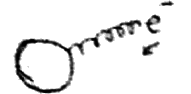
\includegraphics[width=0.2\textwidth]{./images/1-lorentz-model}
	\caption{Diagram of the Lorentz model for an atom}
	\label{fig:lorentz-model}
\end{figure}

Therefore, the equation of motion for the electron is
\begin{align*}
	\ddot{x} + \omega_{0}^{2}x = 0 \qc \omega_{0} = \sqrt{\frac{k}{m}} \Rightarrow x = A \cos(\omega_{0} t + \varphi)
\end{align*}
Introducing a damping term to account for the spontaneous emission, we get
\begin{align}
	\ddot{x} + \gamma \dot{x} + \omega_{0}^{2}x = 0
\end{align}

%-----------------------------------------------------------------
\subsection[Electric dipole approximation]{Electric dipole approximation (EDA)}
In the presence of an external electric field, $\va{E}(z,t) = E_{0} \cos(kz - \omega t) \vu{x}$, and introducing the oscillator strength, $f$, we can explain absorption and stimulated emission as well.

\begin{defi}[Oscillator strength]
	The oscillator strength, $f$, is a dimensionless quantity that expresses the probability of absorption or emission of electromagnetic radiation in transitions between energy levels of an atom or molecule.
	\begin{align*}
		f &> 0 \Rightarrow \text{ absorption} \\
		f &< 0 \Rightarrow \text{ stimulated emission}
	\end{align*}
\end{defi}

The force that acts upon a charged particle in the presence of an electric field is $\va{F} = q \va{E}$, therefore, we get
\begin{align*}
	\ddot{x} + \gamma \dot{x} + \omega_{0}^{2}x = f \frac{e E_{0}}{m} \cos(kz - \omega t)
\end{align*}

We can assume that the size of the atom is much smaller than the optical wavelength, so that the electron only sees the field at the nuclear position; this approximation is the so called electric dipole approximation. Therefore, $k z_{cm} \to 0$, and the previous equation becomes
\begin{align}
	\ddot{x} + \gamma \dot{x} + \omega_{0}^{2}x = f \frac{e E_{0}}{m} \cos(\omega t)
\end{align}

Consequently, we can get absorption or stimulated emission. Since $\dv*{W}{t} = - P$, we can study them measuring the mean value of the power in a cycle:
\begin{align}
	\ev{P} = \ev{F \dot{x}}
	\begin{cases}
		>0 & \text{(absorption)} \\
		<0 & \text{(stimulated emission)}
	\end{cases}
\end{align}
This models gives us $x(t)$.

\subsubsection*{Susceptibility}
In a homogeneous linear and isotropic dielectric medium, the polarization is aligned with and proportional to the electric field: $\va{P} = \varepsilon_{0} \chi \va{E}$. In a dipole, it can be written as $P = N e x$. Therefore, we can express the susceptibility as
\begin{align}
	\chi = \frac{N e x}{\varepsilon E} \equiv \chi' + i \chi''
\end{align}
The real part of the susceptibility, $\Re{\chi} = \chi'$ is related to index of refraction of the medium; the imaginary part, $\Im{\chi} = \chi''$ is related to the absorption coefficient.

\subsubsection*{Other media}
The natural frequency, $\omega_{0}$, gives us the model of the properties of the media. For metals, for instance, $\omega_{0} \to 0$ (electrons are not bound).

%-----------------------------------------------------------------
\subsection{Classical coherence}
\subsubsection*{First-order correlation function}
We can measure the coherence of an electric field with the help of an interferometer. In the figure \ref{fig:interferometer}, we see that $\va{E}_{1} = \va{E}(t)$, $\va{E}_{2} = \va{E}(t + \tau)$, and $\va{E}_{sum} = \va{E}_{1} + \va{E}_{2}$. So that, the intensity detected is $I \propto \ev{\va{E}^{2}_{sum}}$.
\begin{figure}[H]
	\centering
	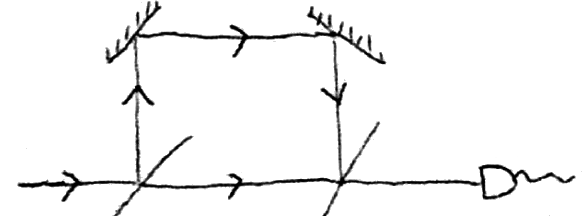
\includegraphics[width=0.5\textwidth]{./images/1-interferometer}
	\caption{Diagram of an interferometer with 50--50 beam splitters}
	\label{fig:interferometer}
\end{figure}

If we express $\va{E}(\va{r},t) = \va{E}^{(-}(\va{r},t) + \va{E}^{(-}(\va{r},t)$, where $\va{E}^{(+)} \equiv \va{E}^{(-)\sast}$, we can rewrite the expression for $I$:
\begin{flalign*}
	I & \propto \ev{(\va{E}_{1} + \va{E}_{2})^{2}} = \cdots = \ev{E^{(-)}_{1} E^{(+)}_{1}} + \ev{E^{(-)}_{2} E^{(+)}_{2}} + 2 \Re{ \ev{E^{(-)}_{1} E^{(+)}_{2}} } & \\
	& \Rightarrow I \propto 2 I_{0} + 2 \Re{E^{(-)}(t) + E^{(+)}(t + \tau)}
\end{flalign*}

\begin{defi}[First-order correlation function]
	\begin{align}
		G^{(1)}(t, t + \tau) \equiv \ev{E^{(-)}(t) + E^{(+)}(t + \tau)} = G^{(1)}(\tau)
	\end{align}
\end{defi}

The visibility is defined as $V = \dfrac{I_{max} - I_{min}}{I_{max} + I_{min}}$. Rewriting the first-order correlation function as $G^{(1)}(\tau) = \abs{G^{(1)}(\tau)} e^{i \phi(\tau)}$, we can easily work out $I_{max}$ and $I_{min}$:
\begin{flalign*}
	I & \propto 2 I_{0} + 2 \abs{G^{(1)}(\tau)} \cos[\phi(\tau)] \Rightarrow
	\begin{cases}
		I[\cos(\phi)] = -1 \Leftrightarrow I_{min} = 2I_{0} - 2 \abs{G^{(1)}(\tau)} \\
		I[\cos(\phi)] = +1 \Leftrightarrow I_{max} = 2I_{0} + 2 \abs{G^{(1)}(\tau)}
	\end{cases}
	 &
\end{flalign*}

\begin{defi}[Normalised first-order coherence function]
	We can rearrange the terms of the visibility to express it in terms of the first-order coherence function:
	\begin{align*}
		V = \dfrac{\abs{G^{(1)}(\tau)}}{\ev{E^{(-)}(t) E^{(+)}(t)}}
	\end{align*}
	this is what we call the normalised first-order coherence function, $g^{(1)}(\tau)$.
	\begin{align}
		V = \frac{I_{max} - I_{min}}{I_{max} + I_{min}} = \abs{g^{(1)}(\tau)}
		\begin{cases}
			= 0 & \Rightarrow \text{incoherent field} \\
			\in (0,1) & \Rightarrow \text{partially coherent field} \\
			= 1 & \Rightarrow \text{fully coherent field}
		\end{cases}
	\end{align}
\end{defi}

\subsubsection*{Second-order correlation function}
\begin{defi}[Normalised second-order correlation function]
	The degree of second-order correlation function is the autocorrelation function for the intensity, rather than the field. We can define this function as
	\begin{align}
		g^{(2)}(\tau) = \frac{\ev{ E^{(-)}(t) E^{(-)}(t + \tau) E^{(+)}(t + \tau) E^{(+)}(t) }}{\ev{ E^{(-)}(t) E^{(+)}(t) }}
	\end{align}
\end{defi}

%-----------------------------------------------------------------
\subsection{Hanbury--Brown--Twiss experiment}
One important feature of the second-order coherence function is that it can be measured with a reasonably simple set-up, the famous Hanbury--Brown–-Twiss apparatus (figure \ref{fig:hbt-experiment}). An input field is divided by a beam splitter, and the two components are monitored by two photo-detectors. The two detector signals are fed into a signal multiplier (mixer), though only after a variable time delay is added to one of the signals. The mixer signal is fed through a low-pass filter, which can be thought of as a integrator with a running time average.
\begin{figure}[H]
	\centering
	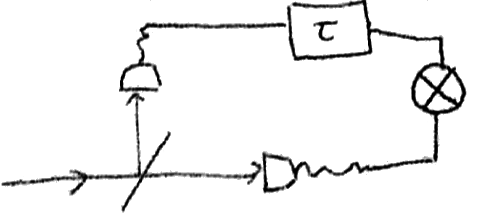
\includegraphics[width=0.4\textwidth]{./images/1-hbt-experiment}
	\caption{Diagram fo the Hanbury--Brown--Twiss experiment}
	\label{fig:hbt-experiment}
\end{figure}
This set-up, because it effectively correlates the two intensities, seems to give the $g^{(2)}(\tau)$ function as its output signal directly:
\begin{align}
	g^{(2)}(\tau) = \frac{\ev{I(t) I(t + \tau)}}{\ev{I(t)}^{2}}
\end{align}

\begin{align*}
	g^{(2)}(\tau)
	\begin{cases}
		\text{stationary field} & g^{(2)} (\tau) = 1 \\
		\text{fluctuating field} &
		\begin{cases}
			g^{(2)} (0) \geq 1 \\
			g^{(2)} (\tau) \leq g^{(2)} (0)
		\end{cases}
		\Rightarrow \text{bunching}
	\end{cases}
\end{align*}

\begin{figure}[H]
	\centering
	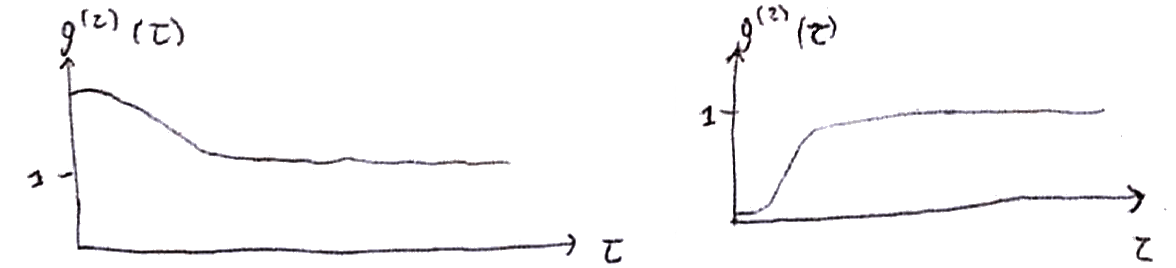
\includegraphics[width=\textwidth]{./images/1-bunching}
	\caption{(a) Bunching in a classical field, (b) antibunching in a quantum field}
	\label{fig:bunching}
\end{figure}

%-----------------------------------------------------------------
%	SEMI-CLASSICAL LIGHT DESCRIPTION
%	!TEX root = ./../main.tex
%----------------------------------------------------------------
\section{Semi-classical light description}
\subsection{Maxwell's equations}
Maxwell's equations are a set of partial differential equations that, together with the Lorentz force Law, form the foundation of classical electrodynamics, classical optics, and electric circuits:
\begin{align}
	\div{D} &= \rho_{free} \tag{Gauss's law} \\
	\div{B} &= 0 \tag{Gauss's law for magnetism} \\
	\curl{E} &= - \pdv{\va{B}}{t} \tag{Faraday's law} \\
	\curl{B} &= \va{J}_{free} + \pdv{\va{D}}{t} \tag{Ampère's law}
\end{align}

Apart from Maxwell's equations themselves, it's important to remember the following relationships for the electric and magnetic fields:
\begin{align*}
	\va{D} = \varepsilon \va{E} + \va{P} \qc \va{B} = \mu_{0} \va{H} + \va{M}
\end{align*}

\subsubsection*{Wave equation}
The general form of the wave wave equation is:
\begin{align*}
	- \laplacian{\va{E}} + \mu_{0} \dv{\va{J}_{free}}{t} + \frac{1}{c^{2}} \dv[2]{\va{E}}{t} = - \mu_{0} \dv[2]{\va{P}}{t}
\end{align*}
However, considering the properties of optical materials ($\rho_{free} = 0$, $\va{M} = \va{0}$, $\mu \approx \mu_{0}$, and $\va{J}_{free} = \va{0}$), we can simplify it and rewrite it as
\begin{align}
	\laplacian{\va{E}} - \frac{1}{c^{2}} \dv[2]{\va{E}}{t} = \mu_{0} \dv[2]{\va{P}}{t}
\end{align}

%-----------------------------------------------------------------
\subsection[Slowly varying envelope approximation]{Slowly varying envelope approximation (SVEA)}
The electric field can be written as
\begin{align}\label{eq:Ezt-epsilon}
	\va{E}(z,t) = \vu{\varepsilon}\, E_{0}(z,t) e^{i(kz - \omega t - \phi(z,t))} = \vu{\varepsilon}\, \mc{E}_{0}(z,t) e^{-i \omega t}
\end{align}
where $\vu{\varepsilon}$ is the unit polarisation vector, and $\mc{E}_{0}$ is the amplitude of the electric field; $E_{0}(z,t)$ and $\phi(z,t)$ are slowly varying functions. Of course, due to a possible phase lag of the medium, the polarization phase may have a phase different from that of the field. In this case, slowly varying means
\begin{align*}
	\left.
	\begin{aligned}
		\abs{\dv{E_{0}}{z}} &\ll \frac{E_{0}}{\lambda} \sim E_{0} k \\
		\abs{\dv{E_{0}}{t}} &\ll \frac{E_{0}}{T} \sim E_{0} \omega
	\end{aligned}
	\right\}
	\qand
	\left\{
	\begin{aligned}
		\abs{\dv{\phi}{z}} &\ll \frac{2 \pi}{\lambda} \sim k \\
		\abs{\dv{\phi}{t}} &\ll \frac{2 \pi}{T} \sim \omega
	\end{aligned}
	\right.
\end{align*}
The slowly varying envelope approximation, thus, is the assumption that the envelope of a forward-travelling wave pulse varies slowly in time and space compared to a period or wavelength. As a result of the slow variation of these functions, when taking derivatives, the highest-order derivatives may be neglected.

Let's consider the wave function in the vacuum, $\dsp \laplacian{\va{E}} - \frac{1}{c^{2}} \dv[2]{\va{E}}{t} = 0$. Since $\va{E} = \va{E}(z,t)$, this becomes
\begin{align}
	\dv[2]{\va{E}}{z} - \frac{1}{c^{2}} \dv[2]{\va{E}}{t} = 0
\end{align}
Following the expression for $\va{E}(z,t)$ in the equation \eqref{eq:Ezt-epsilon}, and deriving the equation above, we get
\begin{align*}
\begin{aligned}
	2i E_{0} (k - \phi') &+ E_{0}'' - i E_{0} \phi'' - E_{0} (k - \phi')^{2} \\
	&= \frac{1}{c^{2}} \qty[ -2i \dot{E}_{0} (\omega + \dot{\phi}) + \ddot{E}_{0} - i E_{0} \ddot{\phi} - E_{0} (\omega + \dot{\phi})^{2}]
\end{aligned}
\end{align*}

Let's apply the slowly varying envelope approximation. On one hand, for the imaginary part of the expression above, we get
\begin{flalign*}
	2 E_{0} \tikzmark{a}k - 2 \tikzmark{b}E_{0} \tikzmark{c}\phi' - E_{0}\tikzmark{d} \phi'' &= \dfrac{1}{c^{2}} \qty[ - 2 \dot{E}_{0} \tikzmark{e}\omega - 2 \tikzmark{f}\dot{E}_{0} \tikzmark{g}\dot{\phi} - i E_{0} \tikzmark{h}\ddot{\phi}] \Rightarrow E_{0}' = - \frac{1}{c} \dot{E}_{0} & \\
	\tikz[overlay,remember picture,label distance=10pt]{\path[draw, <-, square arrow] (a.south) to (b.south); \node[label=below:\footnotesize{SVEA}] at ($ (a) !.5! (b) $) {};}
	\tikz[overlay,remember picture,label distance=10pt]{\path[draw, <-, square arrow] (c.south) to (d.south); \node[label=below:\footnotesize{$\order*{\phi''}$}] at ($ (c) !.5! (d) $) {};}
	\tikz[overlay,remember picture,label distance=10pt]{\path[draw, <-, square arrow] (e.south) to (f.south); \node[label=below:\footnotesize{SVEA}] at ($ (e) !.5! (f) $) {};}
	\tikz[overlay,remember picture,label distance=10pt]{\path[draw, <-, square arrow] (g.south) to (h.south); \node[label=below:\footnotesize{$\order*{\ddot{\phi}}$}] at ($ (g) !.5! (h) $) {};}
\end{flalign*}
On the other hand, for the real part, we get
\begin{flalign*}
	E_{0}'' &- E_{0}(k - \phi')^{2} = \dfrac{1}{c^{2}} \qty[\ddot{E}_{0} - E_{0}(\omega + \dot{\phi})^{2}] \Rightarrow - E_{0} \tikzmark{a}k^{2} + 2 E_{0} k \phi' = \dfrac{1}{c^{2}} \qty[ - E_{0} \tikzmark{b}\omega^{2} - 2 E_{0} \omega \dot{\phi}] & \\
	&\Rightarrow \phi' = - \frac{1}{c} \dot{\phi}
	\tikz[overlay,remember picture,label distance=10pt]{\path[draw, <->, square arrow] (a.south) to (b.south); \node[label=below:\footnotesize{$\equiv$}] at ($ (a) !.5! (b) $) {};}
\end{flalign*}
So, simplifying, and applying the SVEA carefully, we get separate equations for the amplitude and the phase:
\begin{align}
	E_{0}' + \frac{1}{c} \dot{E}_{0} \equiv 0 \qc \phi' + \frac{1}{c} \dot{\phi} \equiv 0
\end{align}

In the presence of a medium, we have to also consider the polarisation. The polarisation can be expressed as $\va{P}(z,t) = \vu{\varepsilon}\, \mc{P}(z,t) e^{i [kz - \omega t - \phi(z,t)]}$, where $\mc{P} \in \mbb{C}$ is the (slowly varying) polarisation amplitude. Having that in mind, and repeating the same process, we get
\begin{align}
	E_{0}' + \frac{1}{c} \dot{E}_{0} = - \frac{k}{2 \varepsilon_{0}} \Im{\mc{P}} \qc E_{0} \qty[\phi' + \frac{1}{c} \dot{\phi}] = - \frac{k}{2 \varepsilon_{0}} \Re{\mc{P}}
\end{align}

\subsubsection*{Steady situation}
In the steady situation, we know that $\dot{E}_{0} = 0$ and $\dot{\phi} = 0$. Also, considering that the polarisation amplitude can be written as $\mc{P}(z) = \varepsilon_{0} \chi E_{0}(z)$, we get
\begin{align}
	\pdv{E_{0}}{z} = - \frac{k}{2} \chi'' E_{0} \qc \pdv{\phi}{z} = - \frac{k}{2} \chi'
\end{align}

\begin{defi}[Absorption coefficient]
	The optical absorption coefficient, $\alpha$ is the most important optical constant
for photo-detectors. Its value is determined by
	\begin{align*}
		\alpha \equiv \frac{i k \chi}{2}
	\end{align*}
\end{defi}

Rewriting the equation for the spatial variation of the electric field in terms of the absorption coefficient we have $E_{0}(z) = E_{0}(0) e^{- \Re{\alpha} z}$. Therefore, we can easily get the Beer's Law:
\begin{align}
	I(z) = I(0) e^{- 2 \Re{\alpha} z}
\end{align}

Since we are in the SVEA regime, we can do a series expansion for the phase: $\phi(z) = \phi(0) + (\dv*{\phi}{z}) z$, therefore, we can rewrite the general phase $\varphi = kz - \omega t - \phi(z)$ as
\begin{flalign*}
	\varphi &= kz - \omega t - \phi (0) + k \frac{\chi'}{2} z = \omega \qty[ \qty(\frac{\chi'}{2}) \frac{z}{c} - t] - \phi(0) \Rightarrow \dd{\varphi} = 0 = \omega \qty[ \qty(\frac{\chi'}{2}) \frac{\dd{z}}{c} - \dd{t}] &
\end{flalign*}

\begin{defi}[Phase velocity]
	The phase velocity of a wave is the rate at which the phase of the wave propagates in space.
	\begin{align}
		v_{ph} \equiv \dv{z}{t} = \frac{c}{1 + \dfrac{\chi'}{2}} = \frac{c}{n (\omega)}
	\end{align}
\end{defi}

%-----------------------------------------------------------------
\subsection{Group velocity}
\begin{defi}[Wave packet]
	A wave packet is a short envelope of localized wave action that travels as a unit. A wave packet can be analysed into, or can be synthesized from, an infinite set of component sinusoidal waves of different wave numbers, with phases and amplitudes such that they interfere constructively only over a small region of space, and destructively elsewhere. For the electric field, it has the following form:
	\begin{align}
		E(z,t) = \int_{\Delta \omega} E_{\omega} e^{i (kz - \omega t)} \dd{\omega} = \underbrace{\qty[\int_{\Delta \omega} E_{\omega} e^{i [(k - k_{0})z - (\omega - \omega_{0})t]} \dd{\omega}]}_{\text{envelope of the amplitude}} \underbrace{e^{i (k_{0}z - \omega_{0} t)}}_{\text{fast oscillation}}
	\end{align}
	where $\Delta k = k - k_{0}$ and $\Delta \omega = \omega - \omega_{0}$.
\end{defi}

\begin{defi}[Group velocity]
	The group velocity of a wave is the velocity with which the overall shape of the waves' amplitudes (known as the modulation or envelope of the wave) propagates through space.
	\begin{align}
		v_{g} = \eval{\frac{\Delta z}{\Delta t}}_{maxima}
	\end{align}
\end{defi}
From the expression for the phase velocity we can see that the wave number can be written as $k = [\omega n(\omega)]/c$. Since the group velocity is defined between two maxima:
\begin{flalign*}
	\pdv{\phi}{\omega} &\equiv 0 = \Delta z \pdv{k}{\omega} - \Delta t \pdv{\omega}{\omega} \Rightarrow v_{g} = \frac{1}{\pdv*{k}{\omega}} \qc \pdv{k}{\omega} = \frac{n}{c} + \pdv{n}{\omega} \frac{\omega}{c} &
\end{flalign*}

Therefore, the group velocity can be written as
\begin{align}
		v_{g} = \frac{c}{\dsp n + \omega \pdv{n}{\omega}}
\end{align}

\subsubsection*{Slow and superluminal light}
Slow and superluminal group velocities can be observed in any material that has large normal ($\pdv*{n}{\omega} > 0$) or anomalous ($\pdv*{n}{\omega} < 0$) dispersion (figure \ref{fig:lorentz-group-vel}):
\begin{itemize}
	\item Superluminal light: $\dsp \pdv{n}{\omega} < 0$.
	\item Slow light: $\dsp \pdv{n}{\omega} > 0$.
\end{itemize}
\begin{figure}[H]
	\centering
	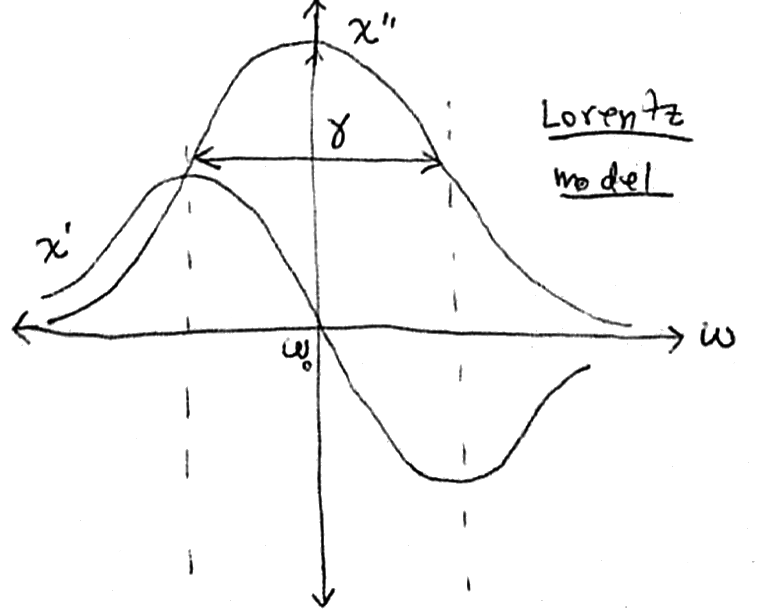
\includegraphics[width=0.6\textwidth]{./images/2-lorentz-group-vel}
	\caption{Slow and superluminal group velocities in the Lorentz model}
	\label{fig:lorentz-group-vel}
\end{figure}

%-----------------------------------------------------------------
%	SEMI-CLASSICAL LIGHT-MATTER INTERACTION
%	!TEX root = ./../main.tex
%----------------------------------------------------------------
\section{Semi-classical light--matter interaction}
\subsection{Basic processes of light--matter interaction}
\begin{figure}[H]
	\centering
	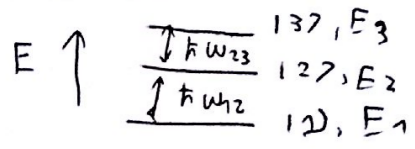
\includegraphics[width=0.4\textwidth]{./images/3-bohr-energies}
	\caption{States and energies in the Bohr model}
	\label{fig:bohr-energies}
\end{figure}

\begin{figure}[H]
	\centering
	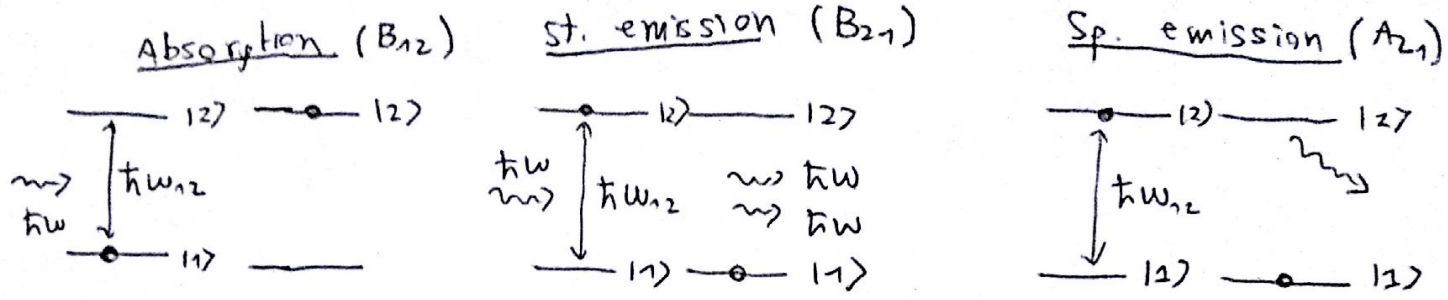
\includegraphics[width=\textwidth]{./images/3-basic-processes}
	\caption{Basic processes of light matter interaction ($\omega \sim \omega_{12}$): (a) absorption, (b) stimulated emission, (c) spontaneous emission}
	\label{fig:basic-processes}
\end{figure}

%-----------------------------------------------------------------
\subsection{Einstein's rate equations}
Let $N_{i}$ be the population of the level $i$. In a closed two-level atom system, $N_{1} + N_{2} = N_{T}$ is constant in time. Therefore,
\begin{align}
	\dv{N_{1}}{t} = \underbrace{- B_{12} N_{1} \rho(\omega)}_{\text{absorption}} + \underbrace{B_{21} N_{2} \rho(\omega)}_{\text{st. emission}} + \underbrace{A_{21} N_{2}}_{\text{sp. em.}} \qc \dv{N_{2}}{t} \equiv - \dv{N_{1}}{t}
\end{align}

%-----------------------------------------------------------------
\subsection{Schrödinger equation}
\begin{defi}[Schrödinger equation]
	In quantum mechanics, the Schrödinger equation is a partial differential equation that describes how the quantum state of a quantum system changes with time. The most general form is the time-dependent Schrödinger equation, which gives a description of a system evolving with time:
	\begin{align}
		i \hbar \pdv{t}\ket{\psi(t)} = H_{0} \ket{\psi(t)} \qc H_{0}\ket{i} = E_{i} \ket{i}
	\end{align}
\end{defi}
Let's consider a time-dependent wave function $\ket{\psi(t)} = \sum_{i} a_{i}(t) e^{-i \omega_{i} t} \ket{i}$, where $\ket{i}$ are eigenstates of the Hamiltonian with eigenenergies $E_{i} = \hbar \omega_{i}$. This wave function satisfies $\abs{\braket{i}{\psi(t)}}^{2} = \abs{a_{i}}^{2}$, $\forall t$.

\subsubsection*{Perturbed Hamiltonian}
When a system is subject to an external interaction or perturbation, the Hamiltonian is corrected by the perturbation Hamiltonian:
\begin{align}
	H = H_{0} + V \qc V \ll H_{0} \quad \Rightarrow i \hbar \pdv{t}\ket{\psi(t)} = (H_{0} + V) \ket{\psi(t)}
\end{align}
From the perturbed Hamiltonian we can derive the temporal evolution of the probability amplitudes $a_{i}$:
\begin{flalign*}
	i \hbar &\sum_{i} (\dot{a}_{i} - i \omega_{i} a_{i}) e^{-i \omega_{i} t} \ket{i} = \sum_{i} (\hbar \omega_{i} + V) a_{i} e^{-i \omega_{i} t} \ket{i} \Rightarrow i \hbar \sum_{i} \dot{a}_{i} e^{-i \omega_{i} t} \ket{i} = \sum_{i} a_{i} e^{-i \omega_{i} t} V \ket{i} & \\
	&\Rightarrow i \hbar \sum_{i} \dot{a}_{i} e^{-i \omega_{i} t} \braket{k}{i} = \sum_{i} a_{i} e^{-i \omega_{i} t} \mel{k}{V}{i} \Rightarrow i \hbar \dot{a}_{k} e^{-i \omega_{k} t} = \sum_{i} \mel{k}{V}{i} a_{i} e^{-i \omega_{i} t}
\end{flalign*}
Therefore, the temporal evolution of the probability amplitude $a_{k}$ is related to the probability amplitudes $a_{i}$:
\begin{align}
	\dot{a}_{k} = - \frac{i}{\hbar} \sum_{i = 1}^{n} \mel{k}{V}{i} a_{i} e^{-i (\omega_{i} - \omega_{k}) t}
\end{align}

\subsubsection*{Two-level atom}
\begin{figure}[H]
	\centering
	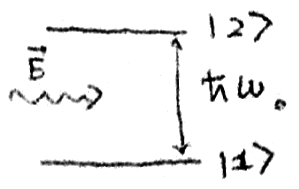
\includegraphics[width=0.25\textwidth]{./images/3-schrodinger-two-level}
	\caption{Two-level atom under an external electric field}
	\label{fig:schrodinger-two-level}
\end{figure}
For a two-level atom, the electric dipole interaction is $V = - \va{\mu} \vdot \va{E}$, where the electric field is $\va{E}(z,t) = \va{E}_{0} \cos(\cancel{kz} - \omega t ) = \va{E}(t)$, and the dipole is\footnote{The reason why $\va{\mu}$ only has off-diagonal elements is because $\va{\mu}_{ij} = e \va{r}_{ij} = \int \va{r} u_{i}(r) u_{j}(r) \dd[3]{r}$. Therefore, the only non-vanishing elements are those coming from states of opposite parity.} $\va{\mu} = \mqty(0 & \va{\mu}_{0} \\ \va{\mu}_{0} & 0)$. Therefore, the temporal evolution of the probability amplitudes is
\begin{subequations}
\begin{align}
	\dot{a}_{1} &= i \Omega \cos(\omega t) e^{-i \omega_{0} t} a_{2} \\
	\dot{a}_{2} &= i \Omega \cos(\omega t) e^{i \omega_{0} t} a_{1}
\end{align}
\end{subequations}
where $\omega_{0} = \omega_{2} - \omega_{1}$, and $\Omega$ is the Rabi frequency. These equations don't have an analytical solution, so we need to introduce the rotating-wave approximation to solve them.

\begin{defi}[Rabi frequency]
	\begin{align}
		\Omega \equiv \frac{\va{\mu}_{0} \vdot \va{E}_{0}}{\hbar} \propto I_{laser}
	\end{align}
\end{defi}

%-----------------------------------------------------------------
\subsection[Rotating-wave approximation]{Rotating-wave approximation (RWA)}
In the rotating-wave approximation, terms in a Hamiltonian which oscillate rapidly are neglected. This is a valid approximation when the applied electromagnetic radiation is near resonance with an atomic transition ($\Omega \ll \omega_{0} \sim \omega$), and the intensity is low. In particular, the probability amplitudes $a_{k}$ are almost constant in comparison with fast oscillating terms (figure \ref{fig:rwa}).
\begin{figure}[H]
	\centering
	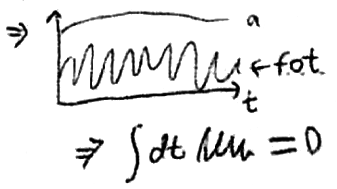
\includegraphics[width=0.3\textwidth]{./images/3-rwa}
	\caption{Comparison between the time dependence of $a_{k}$ and the fast oscillating terms}
	\label{fig:rwa}
\end{figure}

\subsubsection*{Two-level atom under the RWA}
Since $\cos(\omega t) = \qty(e^{i \omega t} + e^{-i \omega t})/2$, we can rewrite the temporal evolution of the probability amplitudes as
\begin{align*}
	\dot{a}_{1} = i \frac{\Omega}{2} \qty\Big[\underbrace{e^{-i (\omega_{0} - \omega) t}}_{\text{slowly osc. term}} + \underbrace{e^{-i (\omega_{0} + \omega) t}}_{\text{fast osc. term}}] a_{2} \qc
	\dot{a}_{2} = i \frac{\Omega}{2} \qty\Big[\underbrace{e^{i (\omega_{0} - \omega) t}}_{\text{slowly osc. term}} + \underbrace{e^{i (\omega_{0} + \omega) t}}_{\text{fast osc. term}}] a_{1}
\end{align*}
where $e^{\pm i (\omega_{0} + \omega) t}$ is fast oscillating term in comparison with $a_{i}$. Therefore, we can apply the RWA and get a simpler expression for the temporal evolution of the probability amplitudes:
\begin{align}\label{eq:rwa-dot-a}
	\dot{a}_{1} = i \frac{\Omega}{2} e^{-i \Delta t} a_{2} \qc \dot{a}_{2} = i \frac{\Omega}{2} e^{i \Delta t} a_{1}
\end{align}
where $\Delta$ is the detuning.

\begin{defi}[Detuning]
	The detuning of the field from the atomic resonance is defined as
	\begin{align}
		\Delta \equiv \omega_{0} - \omega
	\end{align}
\end{defi}

Deriving in both sides of the equation \eqref{eq:rwa-dot-a}, we get a couple of second-order differential equations:
\begin{align*}
	\ddot{a}_{1} + i \Delta \dot{a}_{1} + \qty(\frac{\Omega}{2})^{2} a_{1} = 0 \qc
	\ddot{a}_{2} - i \Delta \dot{a}_{2} + \qty(\frac{\Omega}{2})^{2} a_{2} = 0
\end{align*}
Solving both differential equations we find the following general solutions:
\begin{subequations}
\begin{align}\label{eq:rwa-solutions}
	a_{1}(t) &= A e^{-i (\Delta - \Omega') t/2} + B e^{-i (\Delta + \Omega') t/2} \\
	a_{2}(t) &= C e^{i (\Delta - \Omega') t/2} + D e^{i (\Delta + \Omega') t/2}
\end{align}
\end{subequations}
where $\Omega'$ is the generalised Rabi frequency.

\begin{defi}[Generalised Rabi frequency]
	\begin{align}
		\Omega' \equiv \sqrt{\Omega^{2} + \Delta^{2}}
	\end{align}
\end{defi}

%-----------------------------------------------------------------
\subsection{Rabi oscillations}
For an atom initially in the ground state, $a_{1}(0) = 1$, and $a_{2}(0) = 0$, therefore, $\dot{a}_{1}(0) = 0$, and $\dot{a}_{2}(0) = i \dfrac{\Omega}{2}$. It's not difficult to work out the constants in \eqref{eq:rwa-solutions} and see that
\begin{subequations}
\begin{align}
	a_{1}(t) &= \frac{1}{2 \Omega'} \qty[(\Delta + \Omega') e^{-i (\Delta - \Omega')t/2} + (\Delta - \Omega') e^{-i (\Delta + \Omega')t/2}] \\
	a_{2}(t) &= \frac{\Omega}{2 \Omega'} \qty[ - e^{i (\Delta - \Omega')t/2} + e^{i (\Delta + \Omega')t/2}] = i \frac{\Omega}{\Omega'} e^{i \Delta t/2} \sin(\frac{\Omega'}{2} t)
\end{align}
\end{subequations}

\subsubsection*{Evolution of the populations}
Since the equation for $a_{2}(t)$ is relatively simple, we can calculate the temporal evolution of the populations:
\begin{subequations}
\begin{align}
	P_{2}(t) = a_{2} a_{2}\sast &= \qty(\frac{\Omega}{\Omega'})^{2} \sin[2](\frac{\Omega'}{2} t) \\
	P_{1}(t) = 1 - P_{2}(t) &= 1 - \qty(\frac{\Omega}{\Omega'})^{2} \sin[2](\frac{\Omega'}{2} t)
\end{align}
\end{subequations}
Thus, we see explicitly the significance of the Rabi frequency: the population oscillates between the ground and excited levels at the angular frequency $\Omega$ (figure \ref{fig:rabi-population-p2}). This oscillation phenomenon is referred to as Rabi flopping or Rabi oscillations.
\begin{figure}[H]
	\centering
	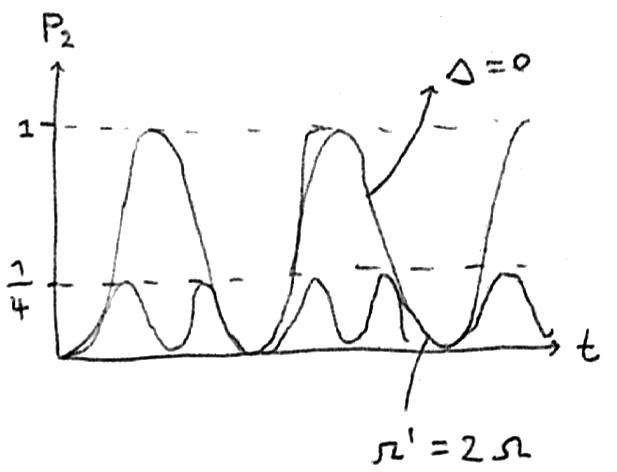
\includegraphics[width=0.5\textwidth]{./images/3-rabi-population-p2}
	\caption{Temporal evolution of the population of the excited state, $P_{2}$}
	\label{fig:rabi-population-p2}
\end{figure}
\begin{example}
	Let's consider the following wave function: $\ket{\psi(t)} = \cos(\frac{\Omega}{2} t) \ket*{\tilde{1}} + i \sin(\frac{\Omega}{2} t) \ket*{\tilde{2}}$, where $\ket*{\tilde{k}} = e^{-i \omega_{k} t} \ket{k}$. Therefore, $\ket{\psi\qty(0)} = \ket*{\tilde{1}}$, $\ket{\psi\qty(\frac{1}{2}\frac{\pi}{\Omega})} = \frac{\sqrt{2}}{2} \ket*{\tilde{1}} + i \frac{\sqrt{2}}{2} \ket*{\tilde{2}}$, $\ket{\psi\qty(\frac{\pi}{\Omega})} = i \ket*{\tilde{2}}$.
\end{example}

\subsubsection*{Electric dipole}
Let's now study the electric dipole in the sense of the Rabi oscillations:
\begin{flalign*}
	\ev{\va{\mu}}{\psi} &= \cdots = a_{1}\sast a_{2} e^{i (\omega_{1} - \omega_{2}) t} \mel{1}{\va{\mu}}{2} + a_{1} a_{2}\sast e^{i (\omega_{2} - \omega_{1}) t} \mel{2}{\va{\mu}}{1} = \va{\mu}_{0} (a_{1}\sast a_{2} e^{-i \omega_{0} t} + a_{1} a_{2}\sast e^{i \omega_{0} t}) &
\end{flalign*}
Therefore, the expected value of the electric dipole is
\begin{align}
	\ev{\va{\mu}}{\psi} = \va{\mu}_{0} \qty{a_{1} a_{2}\sast e^{i \omega_{0} t} + \cc}
\end{align}

\begin{example}
	Let's consider a two-level atom under resonance ($\Delta = 0$), under the effect of an electric dipole and initially in the ground state ($a_{0}(0) = 1$). It's not hard to see that the resulting wave is modulated by the Rabi frequency (figure \ref{fig:rabi-dipole}):
	\begin{align*}
		\ev{\va{\mu}}{\psi} = \va{\mu}_{0} \sin(\Omega t) \sin(\omega_{0} t)
	\end{align*}
	\begin{figure}[H]
		\centering
		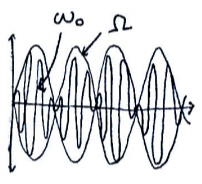
\includegraphics[width=0.25\textwidth]{./images/3-rabi-dipole}
		\caption{Resonance frequency $\omega_{0}$, modulated by the Rabi frequency $\Omega$ in a two-level atom under the effects of an electric dipole}
		\label{fig:rabi-dipole}
	\end{figure}
\end{example}

\subsubsection*{Power absorbed by the atom}
The power absorbed by an atom must be measured as the average of the power over a complete cycle:
\begin{align}
	\ev{P} = \ev{ \va{E}\vdot \dv{t}\ev{\va{\mu_{0}}}_{\psi} } = \frac{\hbar \Omega}{2} \omega \sin(\Omega t)
	% \ev{ \va{E}_{0} \cos(\omega t) \vdot \va{\mu}_{0} \qty[ \cos(\Omega t) \Omega \sin(\omega t) + \sin(\Omega t) \omega \cos(\omega t)] }
\end{align}
\begin{figure}[H]
	\centering
	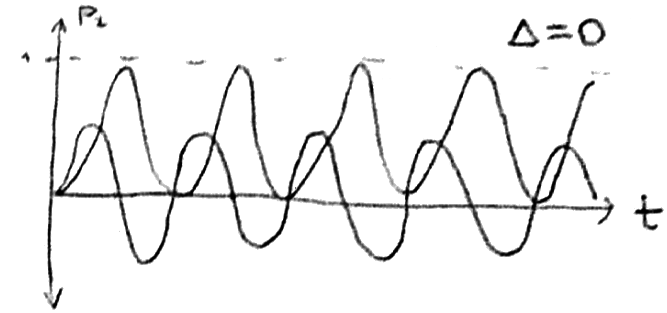
\includegraphics[width=0.6\textwidth]{./images/3-rabi-power}
	\caption{Temporal evolution of the population of the excited state and the power absorbed by an two-level atom. $\ev{P} > 0$ corresponds to the absorption process, while $\ev{P} < 0$ corresponds to stimulated emission}
	\label{fig:rabi-power}
\end{figure}

\subsubsection*{Optical nutation}
% WIP: explain better
Optical nutation is the name given to the transient effect that occurs when a molecular ensemble is suddenly exposed to intense resonant laser light. The molecules undergo alternate absorption and emission of light as they are driven coherently between the upper and lower levels. This results in the intensity of the exciting field being alternately dimed during the absorption phase of the cycle and brightened during the stimulated emission phase.
\begin{figure}[H]
	\centering
	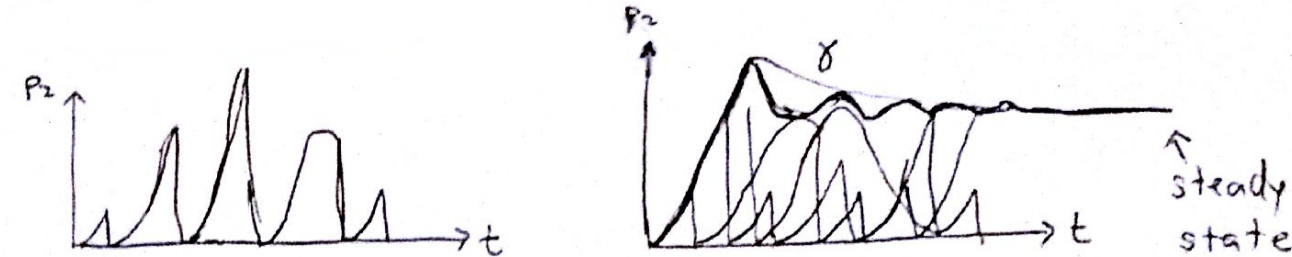
\includegraphics[width=\textwidth]{./images/3-optical-nutation}
	\caption{(a) Quantum jumps in a single atom, (b) optical nutation as the overall effect of $N$ atoms in the absorption phase}
	\label{fig:optical-nutation}
\end{figure}

%-----------------------------------------------------------------
\subsection{AC Stark splitting and dressed atom}
The AC Stark effect is the shifting and splitting of spectral lines of atoms and molecules due to presence of an external electric field. Let's consider a two-level atom; its wave function is $\ket{\psi} = a_{1} e^{-i \omega_{1} t} \ket{1} + a_{2} e^{-i \omega_{2} t} \ket{2}$. The energies are split and shifted:
\begin{subequations}
\begin{align}
	E_{1}^{\pm} &= E_{1} + \hbar \frac{\Delta}{2} \pm \hbar \frac{\Omega'}{2} \\
	E_{2}^{\pm} &= E_{2} - \hbar \frac{\Delta}{2} \pm \hbar \frac{\Omega'}{2}
\end{align}
\end{subequations}

\begin{figure}[H]
	\centering
	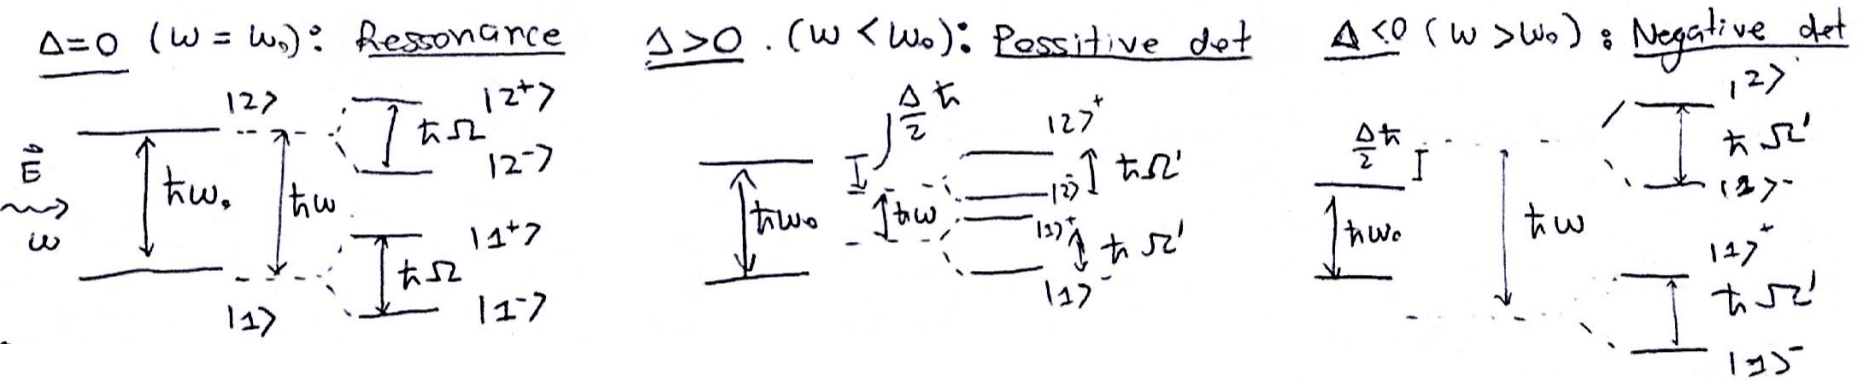
\includegraphics[width=\textwidth]{./images/3-ac-stark-splitting}
	\caption{Diagram of the splitting possibilities: (a) resonance, (b) positive detuning, (c) negative detuning}
	\label{fig:ac-stark-splitting}
\end{figure}

%-----------------------------------------------------------------
\subsection{Mollow triplet}
\begin{figure}[H]
	\centering
	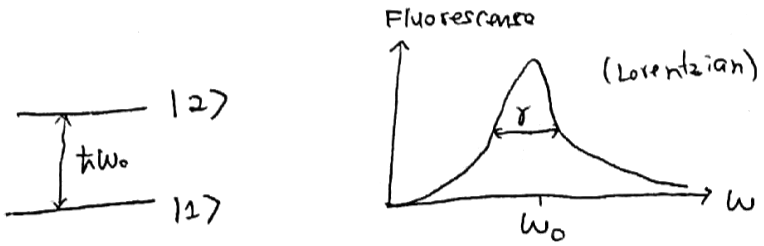
\includegraphics[width=0.7\textwidth]{./images/3-mollow-triplet-pre}
	\caption{Normal behaviour of a two-level atom in the Lorentz model}
	\label{fig:mollow-triplet-pre}
\end{figure}

The Mollow triplet is a very direct manifestation of the dressed-state splittings.

The Mollow triplet (figure \ref{fig:mollow-triplet}) is the lineshape of emission from a two-level atom that is resonantly excited by a continuous wave laser of frequency $\omega$. The triplet that arises from dressing the emitter by the strong laser field is one of the most famous and fundamental spectral lines of quantum optics.
\begin{figure}[H]
	\centering
	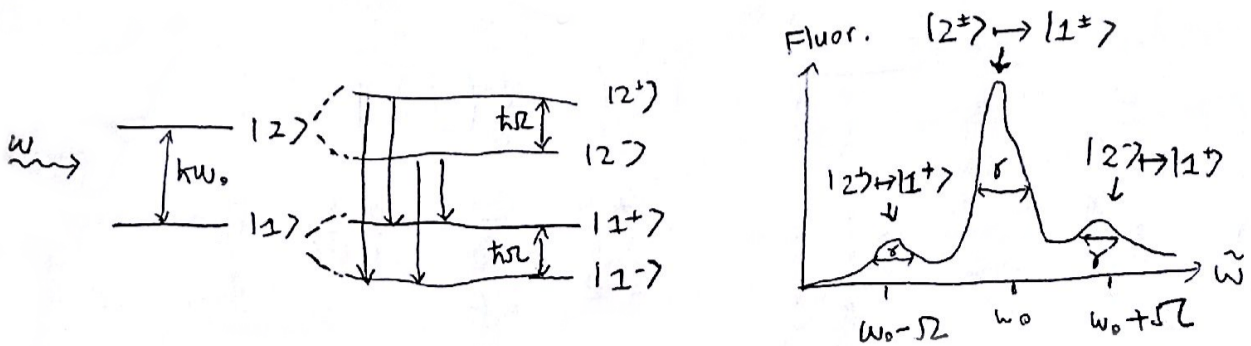
\includegraphics[width=\textwidth]{./images/3-mollow-triplet}
	\caption{Mollow triplet}
	\label{fig:mollow-triplet}
\end{figure}

%-----------------------------------------------------------------
\subsection{Autler--Townes doublet}
\begin{figure}[H]
	\centering
	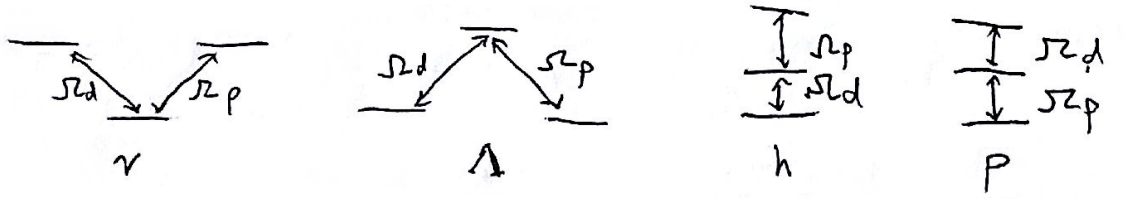
\includegraphics[width=0.9\textwidth]{./images/3-three-level-schemes1}
	\caption{Schemes of possible interactions in a three-level atom, where $\Omega_{d}$ is the due to the drive field, and $\Omega_{p}$ due to a probe field}
	\label{fig:three-level-schemes1}
\end{figure}

The Autler–-Townes doublet is a very direct manifestation of the dressed-state splittings.

Consider the usual two-level atom, driven by a resonant field of Rabi frequency $\Omega$. Now consider a third, auxiliary level $\ket{3}$, an energy $\hbar \omega_{32}$ above the usual excited state $\ket{2}$. We will assume a weak probe field of frequency $\omega_{p}$ coupling $\ket{2} \leftrightarrow \ket{3}$ (such that $\omega_{p} \sim \omega_{32}$). Thus, in the presence of a strong drive (large $\Omega$), the excited state splits into a doublet of splitting $\Omega$ due to mixing with the ground state. Thus, we expect the probe-absorption spectrum to have two peaks, corresponding to resonance of $\ket{3}$ with each of the dressed states. In the limit of large $\Omega$, we expect the absorption spectrum to be a sum of two Lorentzian peaks (figure \ref{fig:autler-townes-doublet}).
\begin{figure}[H]
	\centering
	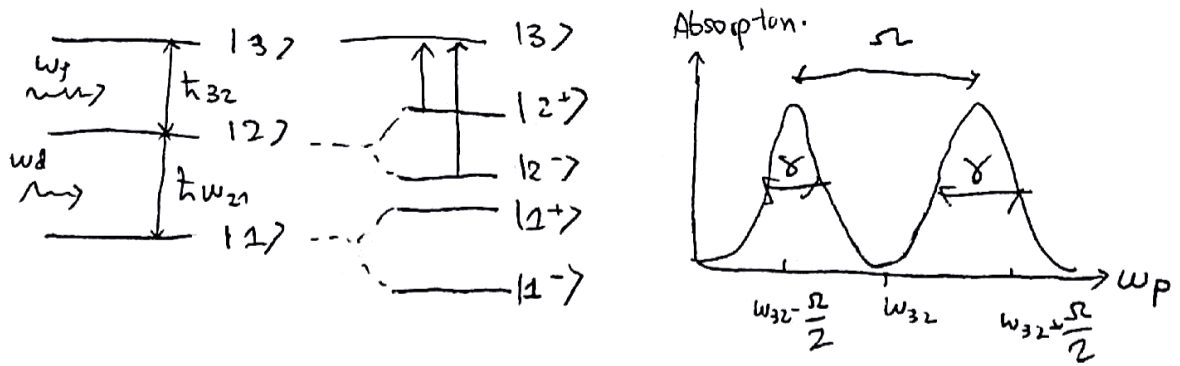
\includegraphics[width=\textwidth]{./images/3-autler-townes-doublet}
	\caption{Autler--Townes doublet}
	\label{fig:autler-townes-doublet}
\end{figure}
If $f(\omega_{32}) = 0$, we have electromagnetically-induced transparency.

%-----------------------------------------------------------------
\subsection{Light shifts and dipole force}
When $\abs{\Delta} \gg \Omega$, we can express the generalised Rabi frequency as $\Omega' = \abs{\Delta} \sqrt{1 + \qty(\frac{\Omega}{\Delta})^{2}} \approx \abs{\Delta } \qty[1 + \frac{1}{2}\qty(\frac{\Omega}{\Delta})^{2}]$. Therefore,
\begin{flalign*}
	E_{1}^{\pm} &= E_{1} + \hbar \frac{\Delta}{2} \pm \hbar \frac{\Omega'}{2} \Rightarrow
	\begin{cases}
		\dsp E_{1}^{+} = E_{1} + \hbar \frac{\Delta}{2} + \hbar \frac{\Delta}{2} + \hbar \frac{1}{4} \frac{\Omega^{2}}{\Delta} & \text{far from } E_{1} \\
		\\
		\dsp E_{1}^{-} = E_{1} + \hbar \frac{\Delta}{2} - \hbar \frac{\Delta}{2} - \hbar \frac{1}{4} \frac{\Omega^{2}}{\Delta} & \text{close to } E_{1}
	\end{cases}
	&
\end{flalign*}
This result means, that one of the level splits (which one depends of the sign of $\Delta$) suffers just a small light shift $\delta E = \hbar \dfrac{\Omega^{2}}{4 \Delta}$ (as seen in the figure \ref{fig:light-shifts}). This results in having a significant energy shift with a negligible population in the excited state (there are no Rabi oscillations).
\begin{figure}[H]
	\centering
	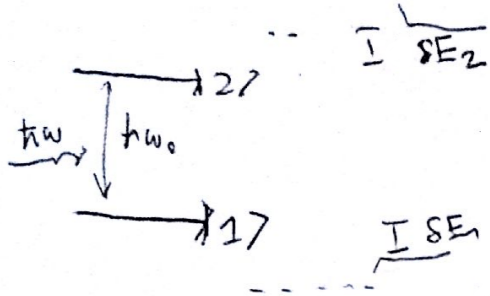
\includegraphics[width=0.4\textwidth]{./images/3-light-shifts}
	\caption{Light shifts, $\delta E$, suffered by the ground and excited states when $\abs{\Delta} \gg \Omega$}
	\label{fig:light-shifts}
\end{figure}

Since $F \propto \grad{I}/\Delta$, we have two possibilities:
\begin{itemize}
	\item Red detuning ($\omega < \omega_{0}$; $\Delta < 0$): the atoms will tend to go to the maxima of $I$.
	\item Blue detuning ($\omega > \omega_{0}$; $\Delta > 0$): the atoms will tend to go to the minima of $I$.
\end{itemize}

%-----------------------------------------------------------------
\subsection{Density matrix formalism}
Let's consider a wave function $\ket{\psi} = \sum_{i} a_{i} \ket{i}$ with probability $p_{\psi}$.
\begin{defi}[Density matrix]
	We define the density matrix as
	\begin{align}
		\rho \equiv \sum_{\psi} p_{\psi} \ketbra{\psi} = \sum_{\psi} p_{\psi} \sum_{i,j} a_{i} a_{k}\sast \ketbra{i}{j}
	\end{align}
\end{defi}

\begin{defi}[Populations and coherences]
	The density matrix elements are
	\begin{align*}
		\rho_{ij} = \braket{i}{\rho}{j} = \sum_{\psi} p_{\psi} a_{i}a_{j}\sast \equiv \overline{a_{i} a_{j}\sast}
	\end{align*}
	We can classify these matrix elements in:
	\begin{itemize}
		\item Populations: $\rho_{ii} = a_{i} a_{i}\sast \in \mbb{R}$.
		\item Coherences $\rho_{ij} = a_{i} a_{j}\sast \in \mbb{C}$, $\forall i \neq j$.
	\end{itemize}
\end{defi}

It's not difficult to calculate the expectation value of an arbitrary operator:
\begin{flalign*}
	\ev{A}_{\psi} & = \ev{A}{\psi} = \sum_{i,j} a_{j} a_{i}\sast A_{ij} & \\
	\ev{A} &= \sum_{\psi} p_{\psi} \ev{A}{\psi} = \cdots = \sum_{ij} \rho_{ij} A_{ji} = \sum_{i} \qty\Big[ \sum_{j} \rho_{ij} A_{ji} ] = \sum_{i} (\rho A)_{ii} \equiv \Tr(\rho A)
\end{flalign*}

\subsubsection*{Equation of motion of the density matrix}
From the definition of the Hamiltonian, we can calculate the temporal evolution of the amplitude probabilities:
\begin{flalign*}
	i \hbar \, \dot{a}_{j} &= \sum_{i} H_{ji} a_{i} \Rightarrow
	\begin{cases}
		\dsp a_{j}\sast \dot{a}_{i} = - \frac{i}{\hbar} a_{j}\sast \sum_{k} H_{ik} a_{k} \\
		\dsp \dot{a}_{j}\sast a_{i} = + \frac{i}{\hbar} a_{i} \sum_{k} H_{jk}\sast a_{k}\sast
	\end{cases} &
\end{flalign*}

From the definition of the matrix elements of the density matrix, $\dsp \rho_{ij} = \sum_{\psi} p_{\psi} a_{j}\sast a_{i}$ and the results we've just gotten from the Hamiltonian, we can calculate its temporal evolution:
\begin{flalign*}
	\dot{\rho}_{ij} &= \sum_{\psi} p_{\psi} \qty( a_{j}\sast \dot{a}_{i} + \dot{a}_{j}\sast a_{i} ) = \frac{i}{\hbar} \sum_{\psi} p_{\psi} \sum_{k} \qty( a_{i} a_{k}\sast H_{kj} - a_{j}\sast a_{k} H_{ik} ) & \\
	&= \frac{i}{\hbar} \sum_{k} \qty( \rho_{ik} H_{kj} - \rho_{kj} H_{ik} ) \equiv - \frac{i}{\hbar} \comm{H}{\rho}_{ij} & \\
\end{flalign*}

\begin{subequations}
This is called the Schrödinger--von Neumann equation:
\begin{align}
	\dot{\rho} = - \frac{i}{\hbar} \comm{H}{\rho}
\end{align}
For incoherent terms, we introduce the Liouville operator, $L$:
\begin{align}
	\dot{\rho} = - \frac{i}{\hbar} \comm{H}{\rho} + L \rho
\end{align}
\end{subequations}

\subsubsection*{Temporal evolution of a two-level atom}
\begin{figure}[H]
	\centering
	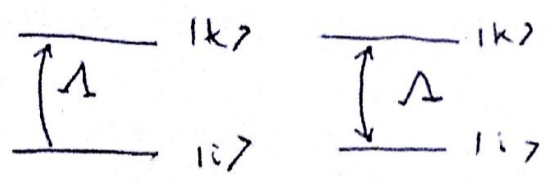
\includegraphics[width=0.35\textwidth]{./images/3-two-level-pumping}
	\caption{Diagram of possible interactions in a two-level atom: (a) unidirectional pumping, (b) bidirectional pumping}
	\label{fig:two-level-pumping}
\end{figure}

The decay of populations by spontaneous emission is
\begin{align*}
	\dot{\rho}_{ii} = - \frac{i}{\hbar} \comm{H}{\rho}_{ii} + \sum_{E_{j}>E_{i}} \Gamma_{ji} \rho_{jj} - \sum_{E_{j}<E_{i}} \Gamma_{ij} \rho_{ii}
\end{align*}
The incoherent pump between levels $\ket{i}$ and $\ket{k}$ due to bidirectional pumping is
\begin{align*}
	\qty(\dot{\rho}_{ii})_{pump} = \Lambda \qty(\rho_{kk} - \rho_{ii}) \qc \qty(\dot{\rho}_{kk})_{pump} = \Lambda \qty(\rho_{ii} - \rho_{kk})
\end{align*}

\subsubsection*{Temporal evolution of a three-level atom}
\begin{figure}[H]
	\centering
	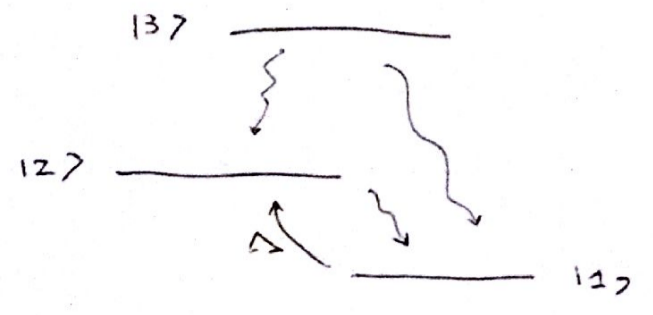
\includegraphics[width=0.5\textwidth]{./images/3-three-level-decay}
	\caption{Diagram of possible interactions in a three-level atom}
	\label{fig:three-level-decay}
\end{figure}

The incoherent terms in the populations are
\begin{align*}
	\qty(\dot{\rho}_{11})_{inc} &= \Gamma_{31} \rho_{33} - \Lambda \rho_{11} + \Gamma_{21} \rho_{22} \\
	\qty(\dot{\rho}_{22})_{inc} &= \Gamma_{32} \rho_{33} + \Lambda \rho_{11} - \Gamma_{21} \rho_{22} \\
	\qty(\dot{\rho}_{33})_{inc} &= - \Gamma_{31} \rho_{33} - \Gamma_{32} \rho_{33}
\end{align*}
As we can see, for a closed system
\begin{align}
	\sum_{i} \qty( \dot{\rho}_{ii} )_{inc} = 0
\end{align}
The incoherent terms in the coherences are
\begin{align*}
	\qty(\dot{\rho}_{ij})_{inc} = - \gamma_{ij} \, \rho_{ij} \geq - \frac{1}{2} \qty\Big[\sum_{i,j} \Gamma_{(i \vee j) k} ] \rho_{ij}
\end{align*}
\begin{example}
	The incoherent terms in $\rho_{23}$ are $\qty(\dot{\rho}_{23})_{inc} = - \dfrac{1}{2} \qty[\Gamma_{32} + \Gamma_{31} + \Gamma_{21}] \rho_{23}$.
\end{example}

\subsubsection*{Temporal evolution of a generic closed atom}
Having in mind both decay by spontaneous emission and pumping processes, we have
\begin{subequations}
\begin{align}
	% \dot{\rho}_{ii} &= - \frac{i}{\hbar} \comm{H}{p}_{ii} + \sum_{E_{j}>E_{i}} \underbrace{(\Gamma_{ji} \rho_{jj} - \Lambda_{ji} \rho_{ii})}_{\text{add}} - \sum_{E_{j}<E_{i}} \underbrace{(\Gamma_{ij} \rho_{ii} - \Lambda_{ij} \rho_{jj} )}_{\text{extract}} \\
	\dot{\rho}_{ii} &= - \frac{i}{\hbar} \comm{H}{\rho}_{ii} + \sum_{k} \underbrace{(\Gamma_{ki} + \Lambda_{ki} ) \rho_{kk}}_{\text{add to } \ket{i}} - \sum_{k} \underbrace{(\Gamma_{ik} + \Lambda_{ik} ) \rho_{ii}}_{\text{extract from } \ket{i}} \\
	\dot{\rho}_{ij} &= - \frac{i}{\hbar} \comm{H}{\rho}_{ij} - \frac{1}{2} \underbrace{\qty\Big[\sum_{i,j} \Gamma_{(i \vee j) k} + \Lambda_{(i \vee j) k} ]}_{\text{extract from } \ket{i} \text{ or } \ket{j}} \rho_{ij}
	% Here \vee means OR
\end{align}
\end{subequations}

%-----------------------------------------------------------------
\subsection{Density matrix for a closed two-level atom}
\begin{figure}[H]
	\centering
	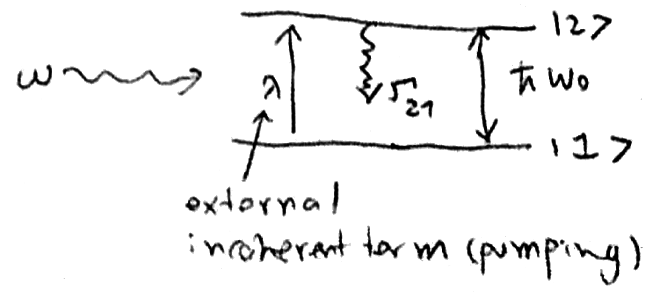
\includegraphics[width=0.45\textwidth]{./images/3-two-level-external}
	\caption{External electric field in a two-level atom}
	\label{fig:two-level-external}
\end{figure}
Since we are in a two-level atom, the density matrix can be expressed as $\rho = \mqty( \rho_{11} & \rho_{12} \\ \rho_{21} & \rho_{22} )$. Also, as we are exposing the system to an external field, the Hamiltonian is $H = H_{0} + V$, where $H_{0}$ is the unperturbed Hamiltonian, and $V = - \va{\mu} \vdot \va{E}$ is the perturbation (or interaction) Hamiltonian:
\begin{align*}
	H_{0} = \hbar \mqty(0 & 0 \\ 0 & \omega_{0}) \qc V = \hbar \mqty( 0 & -\Omega \cos(\omega t) \\ -\Omega \cos(\omega t) & 0 )
\end{align*}
Therefore, the full Hamiltonian can be written as
\begin{align}
	H = \hbar \mqty( 0 & -\Omega \cos(\omega t) \\ -\Omega \cos(\omega t) & \omega_{0} )
\end{align}

\subsubsection*{Going from the Schrödinger picture to the interaction picture}
To go from the Schrödinger picture to the interaction picture we need to make a unitary transformation for the operators and the states. The reason to do this is because $\omega$ is a fast oscillating term and the dynamics are quite tricky. Working in the interaction picture allows us to apply the RWA, making fast oscillating terms vanish from the Hamiltonian. Therefore,
\begin{align}
	\bar{H} = U H U^{-1} \qc \bar{\rho} = U \rho \, U^{-1}
\end{align}
\begin{defi}[Unitary time-evolution operator]
	The unitary matrix $U$ is called the time-evolution operator:
	\begin{align}
		U = \exp[i \dfrac{H_{IP}}{\hbar} t]
	\end{align}
	where $H_{IP}$ is the interaction picture Hamiltonian. Therefore,
	\begin{align*}
		H_{IP} = \hbar \mqty(0 & 0 \\ 0 & \omega) \Rightarrow U = \mqty(1 & 0 \\ 0 & e^{i \omega t})
	\end{align*}
\end{defi}
 Let's work out the expression of $\bar{H}$:
\begin{flalign*}
	\bar{H} &= \hbar \mqty( 0 & -\frac{\Omega}{2}(1 + e^{-i 2 \omega t}) \\ -\frac{\Omega}{2}(1 + e^{-i 2 \omega t}) & \omega_{0} ) \overset{\text{RWA}}{\Longrightarrow} \bar{H} = \hbar \mqty( 0 & -\frac{\Omega}{2} \\ -\frac{\Omega}{2} & \omega_{0} ). &
\end{flalign*}
Let's now work out the behaviour of $\bar{\rho}$:
\begin{flalign*}
	\dot{\bar{\rho}} &= \dv{U}{t} \rho U^{-1} + U \dv{\rho}{t} U^{-1} + U \rho \dv{U^{-1}}{t} = \frac{i H_{IP}}{\hbar} \bar{\rho} + U \qty( - \frac{i}{\hbar} \comm{H}{\rho} ) U^{-1} - \bar{\rho} \frac{i H_{IP}}{\hbar} & \\
	&= - \frac{i}{\hbar} \comm{H_{IP}}{\bar{\rho}} + \frac{i}{\hbar} \comm{\bar{H}}{\bar{\rho}} = -\frac{i}{\hbar} \comm{\bar{H} - H_{IP}}{\bar{\rho}}.
\end{flalign*}
Therefore, we have an explicit expression for $\bar{H}$, and we also have also derived the Schrödinger--von Neumann in the interaction picture\footnote{From now on, even though we will be always working in the interaction picture, we will refer to the density matrix simply as $\rho$ instead of $\bar{\rho}$.}:
\begin{align}
	\bar{H} = \hbar \mqty( 0 & -\frac{\Omega}{2} \\ -\frac{\Omega}{2} & \omega_{0} )
	 \qc \dot{\bar{\rho}} = -\frac{i}{\hbar} \comm{\bar{H} - H_{IP}}{\bar{\rho}}
\end{align}
Therefore, we have
\begin{align*}
	\mqty( \dot{\rho}_{11} & \dot{\rho}_{12} \\ \dot{\rho}_{21} & \dot{\rho}_{22}) &= - \frac{i}{\hbar} \comm{\hbar \mqty( 0 & -\frac{\Omega}{2} \\ -\frac{\Omega}{2} & \Delta )}{\mqty( \rho_{11} & \rho_{12} \\ \rho_{21} & \rho_{22})} \\
	&= i \mqty( \frac{\Omega}{2}(\rho_{21} - \rho_{12}) & \frac{\Omega}{2}(\rho_{22} - \rho_{11}) + \Delta \rho_{12} \\ \frac{\Omega}{2}(\rho_{11} - \rho_{22}) - \Delta \rho_{12} & \frac{\Omega}{2}(\rho_{12} - \rho_{21}) )
\end{align*}
It's important to notice that, just as we wanted, our Hamiltonian ($\bar{H} - H_{IP}$) is written just in terms of the Rabi frequency and the detuning.

Writing the coherences as $\rho_{12} = x_{12} + i y_{12}$ and $\rho_{21} = x_{12} - i y_{12}$, and taking into account both the coherent and incoherent terms, we get
\begin{subequations}
\begin{align}
	\dot{\rho}_{11} &= \Omega \, y_{12} + \Gamma_{21} \rho_{22} \qc \dot{\rho}_{22} = - \dot{\rho}_{11} \\
	\dot{\rho}_{12} &= i \Delta \rho_{12} + i\frac{\Omega}{2} (\rho_{22} - \rho_{11}) - \gamma_{12} \, \rho_{12} \\
	\dot{x}_{12} &= - \Delta y_{12} - \gamma_{12} \, x_{12} \\
	\dot{y}_{12} &= \Delta x_{12} + \frac{\Omega}{2} (\rho_{22} - \rho_{11}) - \gamma_{12} \, y_{12}
\end{align}
\end{subequations}


\subsubsection*{Radiative limit}
The radiative limit is the reason why $\gamma \geq \dfrac{1}{2} [\cdots]$. Taking into account only the processes that extract population, we get
\begin{flalign*}
	(\dot{\rho}_{22})_{rad} &= - \Gamma_{21} \rho_{22} \Rightarrow \dot{a}_{2} a_{2}\sast + a_{2} \dot{a}_{2}\sast = - \Gamma_{21} a_{2} a_{2}\sast & \\
	(\dot{\rho}_{11})_{rad} &= - \lambda \rho_{11} \Rightarrow \dot{a}_{1} a_{1}\sast + a_{1} \dot{a}_{1}\sast = - \lambda a_{1} a_{1}\sast
\end{flalign*}
Assuming that the evolution of the probability amplitudes is linear ($\dot{a}_{i} = - A_{i} a_{i}$), we get
\begin{flalign*}
	- \Gamma_{21} &= - 2 A_{2} \Rightarrow A_{2} = \frac{\Gamma_{21}}{2} \qc - \lambda = - 2 A_{1} \Rightarrow A_{1} = \frac{\lambda}{2} &
\end{flalign*}
Therefore, for the coherences we have
\begin{flalign*}
	(\dot{\rho}_{12})_{rad} &= \dot{a}_{1} a_{2}\sast + a_{1} \dot{a}_{2}\sast = - \frac{\lambda}{2} a_{1} a_{2}\sast - a_{1} \frac{\Gamma_{21}}{2} a_{2}\sast = -\frac{1}{2} (\lambda + \Gamma_{21}) \rho_{12} \equiv - \gamma_{12} \rho_{12}. &
\end{flalign*}

\subsubsection*{Steady state solution}
Let's consider the steady state ($\dot{\rho}_{11} = \dot{\rho}_{22} = \dot{x}_{12} = \dot{y}_{12} = 0$). For these conditions, it's not hard to see that
\begin{align}
	x_{12} = \frac{4 \Omega (\lambda - \Gamma_{21}) \Delta}{\qty[4 \Delta^{2} + 4 \Omega^{2} + (\lambda + \Gamma_{21})^{2}] (\lambda + \Gamma_{21})} \qc y_{12} = \frac{2 \Omega (\lambda - \Gamma_{21})}{4 \Delta^{2} + 4 \Omega^{2} + (\lambda + \Gamma_{21})^{2}}
\end{align}
\begin{itemize}
	\item If $\lambda > \Gamma_{21} \Rightarrow y_{12} > 0$, therefore the population $\rho_{11}$ increases (emission).
	\item If $\lambda < \Gamma_{21} \Rightarrow y_{12} < 0$, therefore the population $\rho_{11}$ decreases (absorption).
\end{itemize}

\begin{figure}[H]
	\centering
	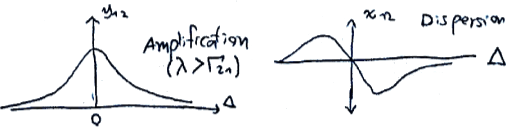
\includegraphics[width=0.6\textwidth]{./images/3-amp-disp}
	\caption{(a) Light amplification and (b) dispersion for $\lambda > \Gamma_{21}$}
	\label{fig:amp-disp}
\end{figure}

%-----------------------------------------------------------------
\subsection{Optical Bloch equations}
\subsubsection*{Bloch sphere}
In quantum mechanics, the Bloch sphere is a geometrical representation of the pure state space of a two-level quantum mechanical system.
\begin{figure}[H]
	\centering
	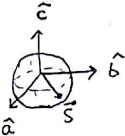
\includegraphics[width=0.2\textwidth]{./images/3-bloch-sphere}
	\caption{Diagram of the Bloch sphere}
	\label{fig:bloch-sphere}
\end{figure}

\begin{defi}[Bloch vector]
	We define the Bloch vector $\va{S}$ as a normal vector in a fictitious space called the Bloch sphere:
	\begin{align}
		\va{S} = u \vu{a} + v \vu{b} + w \vu{c}
	\end{align}
\end{defi}


The Bloch vectors are simply the equations found for the density matrix using a new set of variables:
\begin{subequations}
\begin{align}
	u &= \rho_{21} + \rho_{12} = 2 \Re{\rho_{12}} \\
	v &= i (\rho_{21} - \rho_{12}) = 2 \Im{\rho_{12}} \\
	w &= \rho_{22} - \rho_{11}
\end{align}
\end{subequations}

It's not difficult to see how the Bloch vectors evolve in time:
\begin{subequations}
\begin{align}
	\dot{u} &= -\Delta v \\
	\dot{v} &= \Delta u + \Omega w \\
	\dot{w} &= -\Omega v
\end{align}
\end{subequations}

This vector indicates the point within the Bloch sphere that corresponds to a given mixed state:
\begin{itemize}
	\item If $\va{S} = \vu{c}$, the atom is in the excited state.
	\item If $\va{S} = -\vu{c}$, the atom is in the ground state.
	\item If $\va{S} = \vu{b} \Rightarrow \rho_{22} = \rho_{11}$, the atom is in a superposition of both states.
\end{itemize}

%-----------------------------------------------------------------
\subsection{Density matrix for a closed three-level atom}
\begin{figure}[H]
	\centering
	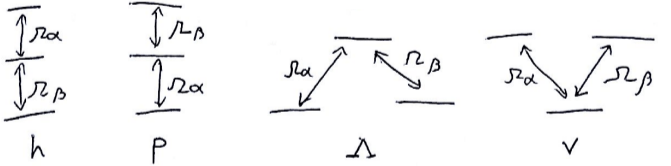
\includegraphics[width=0.7\textwidth]{./images/3-three-level-schemes2}
	\caption{Schemes of possible interactions in a three-level atom, where $\Omega_{\alpha}$ is the due to a weak field, and $\Omega_{\beta}$ due to a strong field}
	\label{fig:three-level-schemes2}
\end{figure}

Let's consider an $h$--cascade scheme (figure \ref{fig:h-scheme}). The detunings are $\Delta_{\alpha} = \omega_{12} - \omega_{\alpha}$, $\Delta_{\beta} = \omega_{23} - \omega_{\beta}$.
\begin{figure}[H]
	\centering
	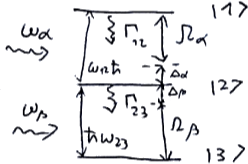
\includegraphics[width=0.33\textwidth]{./images/3-h-scheme}
	\caption{Diagram of an $h$--cascade scheme for a three-level atom}
	\label{fig:h-scheme}
\end{figure}

For constructing the Hamiltonian, we fix the origin of the energy in the state $\ket{3}$. Therefore, we get
\begin{align*}
	H_{0} = \hbar \mqty( \omega_{12} + \omega_{23} & 0 & 0 \\ 0 & \omega_{23} & 0 \\ 0 & 0 & 0 ) \qc V = \hbar \mqty( 0 & - \Omega_{\alpha} \cos(\omega_{\alpha} t) & 0 \\ - \Omega_{\alpha} \cos(\omega_{\alpha} t) & 0 & - \Omega_{\beta} \cos(\omega_{\beta} t) \\ 0 & - \Omega_{\beta} \cos(\omega_{\beta} t) & 0 )
\end{align*}

\subsubsection*{Going from the Schrödinger picture to the interaction picture}
As we've already seen in the two-level atom, to go from the Schrödinger picture to the interaction picture we need to make a unitary transformation for the operators and the states. Therefore,
\begin{align*}
	H_{IP} = \hbar \mqty( \omega_{\alpha} + \omega_{\beta} & 0 & 0 \\ 0 & \omega_{\beta} & 0 \\ 0 & 0 & 0 ) \Rightarrow \bar{H} = U H U^{-1} \overset{\text{RWA}}{=} \hbar \mqty( \omega_{12} + \omega_{23} & -\Omega_{\alpha}/2 & 0 \\ -\Omega_{\alpha}/2 & \omega_{23} & -\Omega_{\beta}/2 \\ 0 & -\Omega_{\beta}/2 & 0 )
\end{align*}

% WIP: trick d'en Jordi amb sumatoris
% Applying\footnote{Jordi's trick:}
Applying the Schrödinger--von Neumann--Liouville equation ($\dot{\bar{\rho}} = - \dfrac{i}{\hbar} \comm{\bar{H} - H_{IP}}{\bar{\rho}} + L \bar{\rho}$), we get the temporal evolutions of the populations and the coherences:
\begin{subequations}
\begin{align}
	\dot{\bar{\rho}}_{11} &= i \frac{\Omega_{\alpha}}{2} (\bar{\rho}_{21} - \bar{\rho}_{12}) - \Gamma_{12} \bar{\rho}_{11} \\
	\dot{\bar{\rho}}_{22} &= i \frac{\Omega_{\alpha}}{2} (\bar{\rho}_{12} - \bar{\rho}_{21}) + i \frac{\Omega_{\beta}}{2} (\bar{\rho}_{32} - \bar{\rho}_{23}) + \Gamma_{12} \bar{\rho}_{11} - \Gamma_{23} \bar{\rho}_{22}\\
	\dot{\bar{\rho}}_{33} &= i \frac{\Omega_{\beta}}{2} (\bar{\rho}_{23} - \bar{\rho}_{32}) + \Gamma_{23} \bar{\rho}_{22}\\
	\dot{\bar{\rho}}_{12} &= i \qty( -\Delta_{\alpha} \bar{\rho}_{12} + \frac{\Omega_{\alpha}}{2} (\bar{\rho}_{22} - \bar{\rho}_{11}) - \frac{\Omega_{\beta}}{2} \bar{\rho}_{13}) - \frac{1}{2}\qty[\Gamma_{12} + \Gamma_{23}] \bar{\rho}_{12} \\
	\dot{\bar{\rho}}_{23} &= i \qty( -\Delta_{\beta} \bar{\rho}_{23} + \frac{\Omega_{\beta}}{2} (\bar{\rho}_{33} - \bar{\rho}_{22}) - \frac{\Omega_{\alpha}}{2} \bar{\rho}_{13}) - \frac{1}{2}\qty[\Gamma_{12} + \Gamma_{23}] \bar{\rho}_{23} \\
	\dot{\bar{\rho}}_{13} &= i \qty( -(\Delta_{\alpha} + \Delta_{\beta}) + \frac{\Omega_{\alpha}}{2} \bar{\rho}_{23} - \frac{\Omega_{\beta}}{2} \bar{\rho}_{12}) - \frac{1}{2}\qty[\Gamma_{12} + \Gamma_{23}] \bar{\rho}_{13}
\end{align}
\end{subequations}


So that, assuming that the atom is a closed system, we need to solve the system to find just $\rho_{11}$, $\rho_{22}$, $x_{12}$, $y_{12}$, $x_{23}$, $y_{23}$, $x_{13}$, and $y_{13}$.

%-----------------------------------------------------------------
\newpage
\subsection[Electromagnetically induced transparency]{Electromagnetically induced transparency (EIM)}
Let's consider a $\Lambda$ scheme (figure \ref{fig:lambda-scheme-eim1}).
\begin{figure}[H]
	\centering
	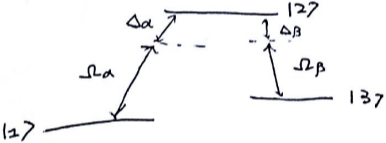
\includegraphics[width=0.5\textwidth]{./images/3-lambda-scheme-eim1}
	\caption{$\Lambda$ scheme for a three-level atom used in the EIM}
	\label{fig:lambda-scheme-eim1}
\end{figure}
It's obvious from the Autler--Townes doublet (figure \ref{fig:eim-abs-disp}) that the absorption, $y_{12}$, cannot be the exact sum of two Lorentzians (the sum of two Lorentzians would only be zero when $\Delta_{\alpha} \to \pm \infty$); so we must consider the quantum interference as well:
\begin{align*}
	y_{12} = (\rho_{22} - \rho_{11}) \cdot 2\text{ Lorentzians} + \text{quantum interference terms}
\end{align*}

Let's now consider the refraction, $x_{12}$. As we can see in the figure \ref{fig:eim-abs-disp}, we can easily modify the group velocity of a medium, which is used for the creation of quantum memories (figure \ref{fig:lambda-scheme-eim2}).
\begin{figure}[H]
	\centering
	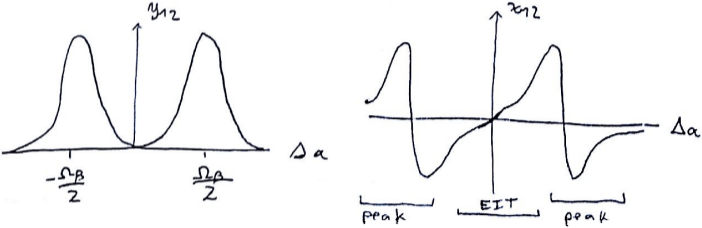
\includegraphics[width=0.8\textwidth]{./images/3-eim-abs-disp}
	\caption{(a) Absorption and (b) refraction of a medium as a function of the detuning of the weak field in the Autler--Townes doublet}
	\label{fig:eim-abs-disp}
\end{figure}

% WIP: expand about quantum memories + caption
\begin{figure}[H]
	\centering
	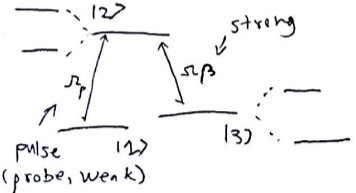
\includegraphics[width=0.45\textwidth]{./images/3-lambda-scheme-eim2}
	\caption{Caption here, something something, quantum memories}
	\label{fig:lambda-scheme-eim2}
\end{figure}

%-----------------------------------------------------------------
\subsection[Coherent population trapping]{Coherent population trapping (CPT)}
The coherent population trapping is only possible for $\Lambda$ schemes (figure \ref{fig:lambda-scheme-cpt}). It's also necessary that $\Delta_{\alpha} = \Delta_{\beta} = \Delta$ (two-photon Raman resonance) and that $\Omega_{\alpha} = \Omega_{\beta} \in \mbb{R}$.
\begin{figure}[H]
	\centering
	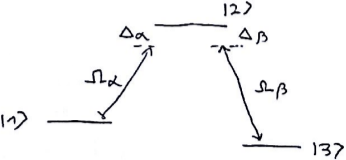
\includegraphics[width=0.5\textwidth]{./images/3-lambda-scheme-cpt}
	\caption{$\Lambda$ scheme for a three-level atom used in the CPT}
	\label{fig:lambda-scheme-cpt}
\end{figure}
The free Hamiltonian and the perturbation are
\begin{align*}
	H_{0} = \hbar \mqty( 0 & 0 & 0 \\ 0 & \omega_{12} & 0 \\ 0 & 0 & \omega_{12} - \omega_{23} ) \qc V = \frac{\hbar}{2} \mqty( 0 & \Omega_{\alpha} e^{i(\omega_{\alpha} t + \phi_{\alpha})} & 0 \\ \Omega_{\alpha} e^{-i(\omega_{\alpha} t + \phi_{\alpha})} & 0 & \Omega_{\beta} e^{-i(\omega_{\beta} t + \phi_{\beta})} \\ 0 & \Omega_{\beta} e^{i(\omega_{\beta} t + \phi_{\beta})} & 0 )
\end{align*}

\begin{defi}[Dark and bright states]
It is useful to define a new basis of states, $\qty{ \ket{D}, \ket{B}, \ket{2}}$, where $\ket{D}$ and $\ket{B}$ are called, respectively, the dark and bright states.
	\begin{subequations}
	\begin{align}
		\ket{D} &= \frac{1}{\bar{\Omega}} \qty[ \Omega_{\beta} e^{i(\omega_{12}t + \phi_{\alpha})} \ket{1} - \Omega_{\alpha}\sast e^{i(\omega_{23}t + \phi_{\beta})} \ket{3}] \\
		\ket{B} &= \frac{1}{\bar{\Omega}} \qty[ \Omega_{\alpha} e^{i(\omega_{12}t + \phi_{\alpha})} \ket{1} + \Omega_{\beta}\sast e^{i(\omega_{23}t + \phi_{\beta})} \ket{3}]
	\end{align}
	\end{subequations}
	where $\bar{\Omega}$ is the Rabi frequency for the $\ket{B} \mapsto \ket{2}$ transition.
\end{defi}

The advantage of using the dark and bright states, and their physical meaning, is that
\begin{align*}
	V \ket{D} = 0 \qc V \ket{B} = \hbar \frac{\bar{\Omega}}{2} e^{i \Delta t} \ket{2}
\end{align*}

\begin{defi}[Rabi frequency for the $\ket{B} \mapsto \ket{2}$ transition]
	\begin{align}
		\bar{\Omega} = \sqrt{ \abs{\Omega_{\alpha}}^{2} + \abs{\Omega_{\beta}}^{2} }
	\end{align}
\end{defi}

Therefore, the $\Lambda$ scheme in this new basis (figure \ref{fig:lambda-dark-bright}) is much simpler than the one seen in the figure \ref{fig:lambda-scheme-cpt}.
\begin{figure}[H]
	\centering
	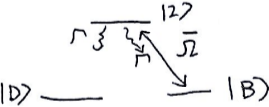
\includegraphics[width=0.33\textwidth]{./images/3-lambda-dark-bright}
	\caption{$\Lambda$ scheme for a three-level atom used in the CPT using the dark and bright states}
	\label{fig:lambda-dark-bright}
\end{figure}

In this scheme we can accumulate all the population (after many cycles) in the dark state.

%-----------------------------------------------------------------
\subsection[Stimulated Raman adiabatic passage]{Stimulated Raman adiabatic passage (STIRAP)}
Now suppose in a three-level atom, you want to move all the population from $\ket{D}$ to $\ket{B}$ using two-photon stimulated Raman transitions.
\begin{figure}[H]
	\centering
	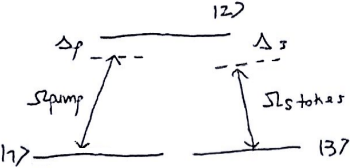
\includegraphics[width=0.45\textwidth]{./images/3-lambda-scheme-stirap}
	\caption{$\Lambda$ scheme for a three-level atom used in the STIRAP}
	\label{fig:lambda-scheme-stirap}
\end{figure}
The Hamiltonian of the $\Lambda$ scheme in the figure \ref{fig:lambda-scheme-stirap} is
\begin{align*}
	H = \frac{\hbar}{2} \mqty( 0 & - \Omega_{p} & 0 \\ - \Omega_{p} & 2 \Delta_{p} & - \Omega_{s} \\ 0 & - \Omega_{s} & 2 (\Delta_{p} - \Delta_{s}) )
\end{align*}
In the case of $\Delta_{p} = \Delta_{s} = \Delta$, we can easily diagonalise the Hamiltonian and get
\begin{subequations}
\begin{alignat}{2}
	\ket{\pm} &= \frac{1}{\sqrt{2}} \qty(\sin \theta \ket{1} \pm \ket{2} + \cos \theta \ket{3}) \qc & \omega^{\pm} &= \pm \frac{1}{2} \sqrt{\Omega_{p}^{2} + \Omega_{s}^{2}} \\
	\ket{D} &= \cos \theta \ket{1} - \sin \theta \ket{3} \qc & \omega^{D} &= 0
\end{alignat}
\end{subequations}
where $\tan \theta \equiv \Omega_{p}/\Omega_{s}$.

The idea is that if you have two laser pulses, one for each optical transition, you should do something counter-intuitive: you should first turn on the laser coupling $\ket{3} \leftrightarrow \ket{2}$ ($\Omega_{s}$), and then later turn on the laser coupling $\ket{1} \leftrightarrow \ket{2}$ ($\Omega_{p}$).

\begin{figure}[H]
	\centering
	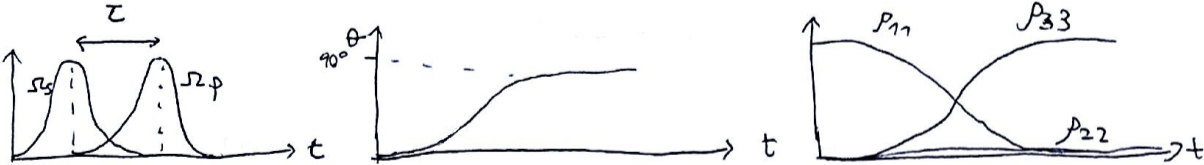
\includegraphics[width=\textwidth]{./images/3-stirap-population}
	\caption{STIRAP: (a) overlap of the pulses, (b) evolution of $\theta$, (c) evolution of the populations}
	\label{fig:stirap-population}
\end{figure}

If we transform the field adiabatically, slowly on time scales of $1/\sqrt{\Omega_{p}^{2} + \Omega_{s}^{2}}$, then the atom will be the dark state, $\ket{D}$, coherently moving all the population from $\rho_{11}$ to $\rho_{33}$.
% \begin{figure}[H]
% 	\centering
% 	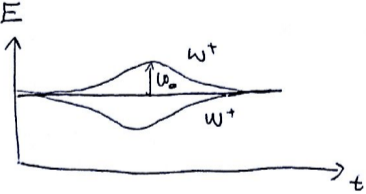
\includegraphics[width=0.35\textwidth]{./images/3-stirap-adiabaticity}
% 	\caption{Caption here, blah blah, adiabaticity, STIRAP}
% 	\label{fig:stirap-adiabaticity}
% \end{figure}

%-----------------------------------------------------------------
%	QUANTUM LIGHT DESCRIPTION
%	!TEX root = ./../main.tex
%-----------------------------------------------------------------
\section{Quantum light description}
\subsection{Classical electrodynamics}
\subsubsection*{Basic equations in the ordinary space}
The basic equations are grouped into two sets. First, the Maxwell equations relate the the electric field $\va{E}(\va{r}, t)$ and the magnetic field $\va{E}(\va{r}, t)$ to the charge density $\rho(\va{r}, t)$ and the current $\va{J}(\va{r}, t)$:
\begin{subequations}
\begin{align}
	\div{E}(\va{r}, t) &= \frac{\rho(\va{r}, t)}{\varepsilon_{0}} \label{eq:max1} \\
	\div{B}(\va{r}, t) &= 0 \label{eq:max2} \\
	\curl{E}(\va{r}, t) &= - \pdv{\va{B}(\va{r}, t)}{t} \label{eq:max3} \\
	\curl{B}(\va{r}, t) &= \frac{1}{c^{2}} \pdv{\va{E}(\va{r}, t)}{t} + \frac{1}{\varepsilon_{0} c^{2}} \va{J}(\va{r}, t) \label{eq:max4}
\end{align}
\end{subequations}
Next, the Newton--Lorentz equation describes the dynamics of each particle $\alpha$ under the influence of electric and magnetic forces exerted by the fields:
\begin{align}
	m_{\alpha} \dv[2]{\va{r}_{a}}{t} = q_{\alpha} \qty[ \va{E}(\va{r}_{\alpha}, t) + \va{v}_{\alpha} \cross \va{B}(\va{r}_{\alpha}, t) ]
\end{align}

The Maxwell's equations implicitly contain the continuity equation ($\pdv*{\rho}{t} + \div{J} \equiv 0$).

The expressions of $\rho(\va{r}, t)$ and $\va{J}(\va{r}, t)$ as a function of the particle variables are
\begin{align}
	\rho(\va{r}, t) &= \sum_{\alpha} q_{\alpha} \delta(\va{r} - \va{r}_{\alpha}(t)) \\
	\va{J}(\va{r}, t) &= \sum_{\alpha} q_{\alpha} \va{v}_{\alpha}(t) \delta(\va{r} - \va{r}_{\alpha}(t))
\end{align}

\subsubsection*{The reciprocal space}
The reciprocal space is the space in which the Fourier transform of a spatial function is represented.
\begin{defi}[Fourier transform]
	A Fourier transform takes us from the ordinary space to the reciprocal space or vice versa:
	\begin{subequations}
	\begin{align}
		\vare{E}(\va{k}, t) &= \frac{1}{(2\pi)^{3/2}} \int \va{E}(\va{r}, t) e^{-i \va{k} \vdot \va{r}} \dd[3]{r} \\
		\va{E}(\va{r}, t) &= \frac{1}{(2\pi)^{3/2}} \int \vare{E}(\va{k}, t) e^{+i \va{k} \vdot \va{r}} \dd[3]{k}
	\end{align}
	\end{subequations}
\end{defi}
% WIP: expand properties?
In this treatment of the space, one frequently uses the following properties of the Fourier transform:
\begin{itemize}
	\item Parseval--Plancherel identity: $\dsp \int F\sast(\va{r}) G(\va{r}) \dd[3]{r} \equiv \int \mc{F}\sast(\va{k}) \mc{G}(\va{k}) \dd[3]{k}$.
	\item Transform of a product (convolution): $\dsp \mc{F}(\va{k})\mc{G}(\va{k}) \leftrightarrow \frac{1}{(2\pi)^{2/3}} \int F(\va{r}\,') G(\va{r} - \va{r}\,') \dd[3]{r'}$.
\end{itemize}

\subsubsection*{Basic equations in the reciprocal space}
Since the $\vnabla$ operator in ordinary space transforms into multiplication by $i \va{k}$ in reciprocal space, Maxwell's equations in reciprocal space become:
\begin{subequations}
\begin{align}
	i\va{k} \vdot \vare{E}(\va{r}, t) &= \frac{\varrho(\va{r}, t)}{\varepsilon_{0}} \\
	i\va{k} \vdot \vare{B}(\va{r}, t) &= 0 \\
	i\va{k} \cross \vare{E}(\va{r}, t) &= - \dot{\vare{B}}(\va{r}, t) \\
	i\va{k} \cross \vare{B}(\va{r}, t) &= \frac{1}{c^{2}} \dot{\vare{E}}(\va{r}, t) + \frac{1}{\varepsilon_{0} c^{2}} \vare{J}(\va{r}, t)
\end{align}
\end{subequations}
The Maxwell's equations implicitly contain the continuity equation ($\dot{\varrho} + i\va{k} \vdot \vare{J} \equiv 0$).

\subsubsection*{Reality condition}
\begin{itemize}
	\item In the ordinary space, a vectorial field is real $\Leftrightarrow \va{E}(\va{r},t) = \va{E}\sast(\va{r},t)$.
	\item In the reciprocal space, a vectorial field is real $\Leftrightarrow \vare{E}(\va{k},t) = \vare{E}\sast(-\va{k},t)$.
\end{itemize}

\subsubsection*{Longitudinal and transverse fields}
Before continuing, it is convenient to distinguish between transverse and longitudinal part of a vector field.
\begin{thm}[Helmholtz theorem]
	For an arbitrary field $\va{V}(\va{r})$, or $\vare{V}(\va{k})$ in the reciprocal space, the Helmholtz theorem states that there is a unique decomposition
	\begin{align}
		\va{V}(\va{r}) = \lng{\va{V}}(\va{r}) + \trn{\va{V}}(\va{r}) \qc \vare{V}(\va{k}) = \lng{\vare{V}}(\va{k}) + \trn{\vare{V}}(\va{k})
	\end{align}
	such that the transverse field is divergence-less
	\begin{align}
		\trn{\div{V}}(\va{r}) = 0 \qc i\va{k} \vdot \trn{\vare{V}}(\va{k}) = 0
	\end{align}
	and the longitudinal field is irrotational
	\begin{align}
		\lng{\curl{V}}(\va{r}) = \va{0} \qc i\va{k} \cross \lng{\vare{V}}(\va{k}) = \va{0}
	\end{align}
\end{thm}

\subsubsection*{Longitudinal electric and magnetic fields}
In the reciprocal space, taking into account the Maxwell's equations and the longitudinal field conditions it's not hard to find an expression for $\lng{\vare{E}}(\va{k})$ and see that the magnetic field is purely transverse:
\begin{align}
	\lng{\vare{E}}(\va{k}) \equiv - \frac{i}{\varepsilon_{0}} \varrho (\va{k}) \frac{\vu{k}}{k} \qc \vare{B}(\va{k}) \equiv \trn{\vare{B}}(\va{k})
\end{align}

Let's now work out the expression for the electric field in the ordinary space:
\begin{flalign*}
	\lng{\va{E}}(\va{r}) & = \mc{F}_{\va{r}}^{-1} \qty{\lng{\vare{E}}(\va{k})} = \mc{F}_{\va{r}}^{-1} \qty{\varrho(\va{k}) \qty(\frac{-i \vu{k}}{\varepsilon_{0} \va{k}})} = \int \rho(\va{r}\,') \frac{1}{4 \pi \varepsilon_{0}} \frac{\va{r} - \va{r}\,'}{\norm{\va{r} - \va{r}\,'}^{3}} \dd[3]{r'}. &
\end{flalign*}
Since charge density is defined as $\rho(\va{r}) \equiv \sum_{\alpha} q_{\alpha} \delta(\va{r} - \va{r}_{\alpha})$, we find the expression of the Coulomb field:
\begin{align}
	\lng{\va{E}}(\va{r}) = \frac{1}{4 \pi \varepsilon_{0}} \sum_{\alpha} q_{\alpha} \frac{\va{r} - \va{r}_{\alpha}}{\norm{\va{r} - \va{r}_{\alpha}}^{3}}
\end{align}
Therefore this is not important to the evolution of the electric field itself; it's just related to the particles.

\subsubsection*{Transverse electric and magnetic fields}
In the reciprocal space, taking into account the Maxwell's equations and the transverse field conditions it's not hard to find expressions for the temporal evolution of $\vare{B}$ and $\trn{\vare{E}}$:
\begin{align}
	\trn{\dot{\vare{E}}} = i c^{2} \va{k} \cross \vare{B} - \frac{1}{\varepsilon_{0}} \trn{\vare{J}} \qc \dot{\vare{B}} = - i \va{k} \cross \trn{\vare{E}}
\end{align}

Apart from that, we can also derive the continuity equation in the reciprocal space:
\begin{flalign*}
	\frac{\lng{\dot{\vare{E}}}}{c^{2}} + \frac{1}{\varepsilon_{0} c^{2}} \lng{\vare{J}} &= 0 \Rightarrow \va{k} \vdot \lng{\dot{\vare{E}}} + \frac{1}{\varepsilon_{0}} \va{k} \vdot (\lng{\vare{J}} + \trn{\vare{J}}) = 0 \Rightarrow \dot{\varrho} + i\va{k} \vdot \vare{J} \equiv 0. &
\end{flalign*}

\subsubsection*{Normal variables}
Let's assume for a moment (for the sake of simplification) that $\trn{\vare{J}} = \va{0}$. Multiplying $\va{k}$ vectorially with the expression we found for the temporal evolution of the magnetic field (and keeping in mind that $\va{A} \cross \va{B} \cross \va{C} = \va{A} (\va{B} \vdot \va{C}) - \va{C} (\va{A} \vdot \va{B})$), we get
\begin{flalign*}
	\va{k} \cross (\dot{\vare{B}} &= - i \va{k} \cross \trn{\vare{E}}) \Rightarrow \va{k} \cross \dot{\vare{B}} = i k^{2} \trn{\vare{E}} &
\end{flalign*}
Mixing this result with the expression for the temporal evolution of the transverse electric field, we get
\begin{align*}
	\pdv{t} \qty( \trn{\vare{E}} \pm c \vu{k} \cross \vare{B}) = \pm i c k \qty( \trn{\vare{E}} \pm c \vu{k} \cross \vare{B})
\end{align*}

One is then led to define, even if $\trn{\vare{J}} \neq \va{0}$, two new variables $\va{\alpha}(\va{k}, t)$ and $\va{\beta}(\va{k}, t)$.

\begin{defi}[Normal variables]
	\begin{subequations}
	\begin{align}
		\va{\alpha}(\va{k}, t) &\equiv - \frac{i}{2 N(k)} \qty[ \trn{\vare{E}} - c \va{k} \cross \vare{B} ] \\
		\va{\beta}(\va{k}, t) &\equiv - \frac{i}{2 N(k)} \qty[ \trn{\vare{E}} + c \va{k} \cross \vare{B} ]
	\end{align}
	\end{subequations}
	where $N(k)$ is a normalisation factor which will be chosen later. The real character of $\trn{\vare{E}}$ and $\vare{B}$ requires that $\va{\beta}(\va{k}, t) \equiv \va{\alpha}\sast(-\va{k}, t) = \va{\alpha}_{-}\sast$. Therefore we can forget about $\va{\beta}$ and write everything in terms of $\va{\alpha}$.
\end{defi}

Since $\va{\alpha}$ is (like $\trn{\vare{E}}$ and $\vare{B}$) a transverse vector field, one can, for each value of $\va{k}$, expand $\va{\alpha}(\va{k},t)$ on two unit vectors $\vu{\epsilon}$ and $\vu{\epsilon}'$, normal to each other and both located in the plane perpendicular to propagation vector. Therefore, we can always write the normal vector as
\begin{align}
	\va{\alpha}(\va{k}, t) \equiv \sum_{\epsilon} \alpha_{\epsilon}(\va{k}, t) \vu{\epsilon}
\end{align}
where $\vu{\epsilon}$ is the transverse polarisation vector, and $\alpha_{\epsilon}(\va{k}, t)$ is the projection of $\va{\alpha}$ into $\vu{\epsilon}$.

Let's rewrite the transverse expression for the electric and the magnetic fields in terms of the normal variables:
\begin{subequations}
\begin{align}
	\trn{\vare{E}} &= i N(k) \qty[ \va{\alpha} - \va{\alpha}_{-}\sast ] \\
	\vare{B} &= \frac{i N(k)}{c} \qty[ \vu{k} \cross \va{\alpha} + \vu{k} \cross \va{\alpha}_{-}\sast ]
\end{align}
\end{subequations}

\subsubsection*{Evolution of the normal variable}
\begin{align}
	\dot{\va{\alpha}} + i \omega \va{\alpha} = \dfrac{i}{2 \varepsilon_{0} N(k)} \trn{\vare{J}}
\end{align}
This can be interpreted as an harmonic oscillator (with $\omega \equiv ck$). Therefore, to completely describe a system at $t_{0}$, we only need to know $\qty{\va{\alpha}(\va{k}, t_{0}), \va{r}_{\alpha}(t_{0}), \va{v}_{\alpha}(t_{0})}$.

\subsubsection*{Energy in terms of the normal variable}
The energy can be defined as the sum of the kinetic and potential energies:
\begin{align}
	H = \sum_{\alpha} \frac{1}{2} m_{\alpha} v^{2}_{\alpha} (t) + \frac{\varepsilon_{0}}{2} \int \qty(E^{2} + c^2 B^{2}) \dd[3]{r}
\end{align}
Let's simplify the terms of the potential energy:
\begin{flalign*}
	\frac{\varepsilon_{0}}{2} \int E^{2} \dd[3]{r} &= \frac{\varepsilon_{0}}{2} \int \qty(\lng{\va{E}} + \trn{\va{E}})^{2} \dd[3]{r} = \frac{\varepsilon_{0}}{2} \int \qty(\lng{E}^{2} + \trn{E}^2 + \cancel{2 \lng{\va{E}} \vdot \trn{\va{E}}}) \dd[3]{r} & \\
	&\Rightarrow \frac{\varepsilon_{0}}{2} \int \qty(E^{2} + c^2 B^{2}) \dd[3]{r} = \underbrace{\frac{\varepsilon_{0}}{2} \int \lng{E}^{2} \dd[3]{r}}_{\lng{H}, \text{ longitudinal}} + \underbrace{\frac{\varepsilon_{0}}{2} \int \qty(\trn{E}^2 + c^{2} B^{2}) \dd[3]{r}}_{\trn{H}, \text{ transverse}} \\
\end{flalign*}
The Coulomb and transverse parts of the potential energy can be simplified further:
\begin{flalign*}
	\lng{H} &= \frac{\varepsilon_{0}}{2} \int \lng{E}^{2} \dd[3]{r} \overset{\text{P. Id.}}{=} \frac{\varepsilon_{0}}{2} \int \lng{\vare{E}}\sast \lng{\vare{E}} \dd[3]{k} = \frac{1}{2 \varepsilon_{0}} \int \varrho\sast(\va{k}) \frac{\varrho(\va{k})}{k^{2}} \dd[3]{k} \qc \varrho(\va{k}) = \sum_{\alpha} \frac{q_{\alpha}}{(2\pi)^{3/2}} e^{-i \va{k} \vdot \va{r}_{\alpha}} & \\
	&\Rightarrow \lng{H} = \sum_{\alpha \neq \beta} \frac{q_{\alpha} q_{\beta}}{2 \varepsilon_{0} (2 \pi)^{3}} \int \frac{e^{-i \va{k} \vdot (\va{r}_{\alpha} - \va{r}_{\beta})}}{k^{2}} \dd[3]{k} = \frac{1}{8 \pi \varepsilon_{0}} \sum_{\alpha \neq \beta} \frac{q_{\alpha} q_{\beta}}{\norm{\va{r}_{\alpha} - \va{r}_{\beta}}} \equiv H_{C} \\
	\trn{H} &= \frac{\varepsilon_{0}}{2} \int \qty(\trn{E}^2 + c^{2} B^{2}) \dd[3]{r} = \frac{\varepsilon_{0}}{2} \int \qty(\trn{\va{E}}\sast \vdot \trn{\va{E}} + c^{2} \va{B}\sast \vdot \va{B}) \dd[3]{r} \\
	&\overset{\text{P. Id.}}{=} \frac{\varepsilon_{0}}{2} \int \qty(\trn{\vare{E}}\sast \vdot \trn{\vare{E}} + c^{2} \vare{B}\sast \vdot \vare{B}) \dd[3]{r} = \varepsilon_{0} \int N^{2} \qty( \va{\alpha}\sast \vdot \va{\alpha} + \va{\alpha}_{-} \vdot \va{\alpha}_{-}\sast ) \dd[3]{k} \\
	&= \varepsilon_{0} \int N^{2} \qty( \va{\alpha}\sast \vdot \va{\alpha} + \va{\alpha} \vdot \va{\alpha}\sast ) \dd[3]{k} = \varepsilon_{0} \int \frac{\hbar \omega}{2} \qty( \va{\alpha}\sast \vdot \va{\alpha} + \va{\alpha} \vdot \va{\alpha}\sast ) \dd[3]{k}
\end{flalign*}
where we have defined the normalisation factor as $N(k) \equiv \sqrt{\dfrac{\hbar \omega}{2}}$.

Therefore, we have seen that the energy can be expressed in a more compact way:
\begin{subequations}
\begin{align}
	H = \sum_{\alpha} \frac{1}{2} m_{\alpha} v^{2}_{\alpha} (t) + H_{C} + \trn{H}
\end{align}
where the Coulomb (or longitudinal) and transverse potentials can be respectively written as
\begin{align}
	H_{C} = \frac{1}{8 \pi \varepsilon_{0}} \sum_{\alpha \neq \beta} \frac{q_{\alpha} q_{\beta}}{\norm{\va{r}_{\alpha} - \va{r}_{\beta}}} \qc \trn{H} = \varepsilon_{0} \int \frac{\hbar \omega}{2} \qty( \va{\alpha}\sast \vdot \va{\alpha} + \va{\alpha} \vdot \va{\alpha}\sast ) \dd[3]{k}
\end{align}
\end{subequations}
From the expression of $\trn{H}$, one can think of the electromagnetic field can be as the sum of harmonic oscillators of frequency $\omega$ being associated with each pair of vectors $\va{k}$, $\vu{\epsilon}$. Such a pair defines a mode of the transverse field.

\subsubsection*{Linear momentum in terms of the normal variable}
The total linear momentum is the sum of the particle mechanical momenta $m_{\alpha} \va{v}_{\alpha}$ and the field momentum:
\begin{subequations}
\begin{align}
	\va{P} = \sum_{\alpha} m_{\alpha} \va{v}_{\alpha} + \varepsilon_{0} \int \qty(\va{E} \cross \va{B}) \dd[3]{r}
\end{align}

Having in mind that $\va{E} = \lng{\va{E}} + \trn{\va{E}}$, doing a calculation similar to that for $\trn{H}$, we can find an expression for the the transverse part of the linear momentum:
\begin{align}
	\trn{\va{P}} = \varepsilon_{0} \int \qty(\trn{\va{E}} \cross \va{B}) \dd[3]{r} = \int \frac{\hbar \va{k}}{2} \qty(\va{\alpha}\sast \vdot \va{\alpha} + \va{\alpha} \vdot \va{\alpha}\sast) \dd[3]{k}
\end{align}
\end{subequations}

\subsubsection*{Electric and magnetic fields in ordinary space}
To find the expression for the electric field in the ordinary space we just need to apply the inverse Fourier transform:
\begin{flalign*}
		\trn{\va{E}}(\va{r}, t) &\equiv \frac{1}{(2\pi)^{3/2}} \int \trn{\vare{E}}(\va{k}, t) e^{i \va{k} \vdot \va{r}} \dd[3]{k} = \int \sqrt{\frac{\hbar \omega}{2 \varepsilon_{0}}} \frac{i}{(2\pi)^{3/2}} \qty(\va{\alpha} - \va{\alpha}_{-}\sast) e^{i \va{k} \vdot \va{r}} \dd[3]{k} & \\
		&= \int \sqrt{\frac{\hbar \omega}{2 \varepsilon_{0}}} \frac{i}{(2\pi)^{3/2}} \sum_{\epsilon} \qty(\alpha_{\epsilon} \vu{\epsilon} \, e^{i \va{k} \vdot \va{r}} - \alpha_{\epsilon -}\sast \vu{\epsilon} \, e^{i \va{k} \vdot \va{r}}) \dd[3]{k} \\
		&= \int \sqrt{\frac{\hbar \omega}{2 \varepsilon_{0}}} \frac{i}{(2\pi)^{3/2}} \sum_{\epsilon} \qty(\alpha_{\epsilon} \vu{\epsilon} \, e^{i \va{k} \vdot \va{r}} - \alpha_{\epsilon}\sast \vu{\epsilon} \, e^{-i \va{k} \vdot \va{r}}) \dd[3]{k} \\
\end{flalign*}
Therefore, the transverse electric field in the ordinary space is
\begin{subequations}
\begin{align}
	\trn{\va{E}}(\va{r}, t) = i \int \sum_{\epsilon} \mc{E}_{\omega} \qty(\alpha_{\epsilon}(\va{k}, t) \vu{\epsilon} \, e^{i \va{k} \vdot \va{r}} - \alpha_{\epsilon}\sast(\va{k}, t) \vu{\epsilon} \, e^{-i \va{k} \vdot \va{r}}) \dd[3]{k}
\end{align}
where $\mc{E}_{\omega} \equiv \dfrac{1}{(2\pi)^{3/2}}\sqrt{\dfrac{\hbar \omega}{2 \varepsilon_{0}}}$ is the amplitude of the reciprocal electric field.

For the magnetic field in the ordinary space we get a similar expression:
\begin{align}
	\trn{\va{B}}(\va{r}, t) = i \int \sum_{\epsilon} \mc{B}_{\omega} \qty(\alpha_{\epsilon}(\va{k}, t) \vu{k} \cross \vu{\epsilon} \, e^{i \va{k} \vdot \va{r}} - \alpha_{\epsilon}\sast(\va{k}, t) \vu{k} \cross \vu{\epsilon} \, e^{-i \va{k} \vdot \va{r}}) \dd[3]{k}
\end{align}
\end{subequations}
where $\mc{B}_{\omega} \equiv \dfrac{\mc{E}_{\omega}}{c}$ is the amplitude of the reciprocal magnetic field.

\subsubsection*{Vector potential}
We can express the electric and the magnetic fields in term of the vector potential:
\begin{align}
	\va{E}(\va{r},t) = - \dv{\va{A}(\va{r},t)}{t} - \grad{U}(\va{r},t) \qc \va{B}(\va{r},t) = \curl{A}(\va{r},t)
\end{align}

Choosing the Coulomb gauge ($\div{A} \equiv 0$), we see that the vector potential is purely transverse. Therefore, it's quite obvious that
\begin{align*}
	\trn{\va{E}} = - \dv{\trn{\va{A}}}{t} \qc \lng{\va{E}} = - \grad{U}
\end{align*}

We can also find the expressions for the the electric and magnetic fields in the reciprocal space:
\begin{align*}
	\trn{\vare{E}} = - \trn{\dot{\vare{A}}} \qc \vare{B} = i \va{k} \cross \trn{\vare{A}}
\end{align*}
Therefore, the transverse vector potential can be written as
\begin{align}
	\trn{\vare{A}} \equiv \sqrt{\frac{\hbar}{2 \varepsilon_{0} \omega}} \qty(\va{\alpha} + \va{\alpha}_{-}\sast)
\end{align}

This expression makes possible to find the normal vector, $\va{\alpha}$, as a function of $\trn{\vare{A}}$ and $\trn{\vare{E}}$:
\begin{align}
	\va{\alpha}(\va{k},t) = \frac{1}{2 N(k)} \qty[\omega \trn{\vare{A}}(\va{k},t) - i \trn{\vare{E}}(\va{k},t)]
\end{align}

\subsubsection*{Periodic boundary conditions}
A useful mathematical trick to quantise the fields is to define a cube of lateral size $L$ and impose periodic boundary conditions:
\begin{align*}
	\trn{\va{E}}(\va{r} + \vu{x} L) = \trn{\va{E}}(\va{r} + \vu{y} L) = \trn{\va{E}}(\va{r} + \vu{z} L)
\end{align*}
In this way $\va{k}$ becomes discrete: $\va{k}_{x,y,z} = \dfrac{2\pi}{L} \vu{k}_{x,y,z}$.

Therefore, we can rewrite everything in terms of the discrete $\va{k}_{r}$:
\begin{align}\label{eq:disc-cont}
	\sum_{\va{k}_{j}} \qty(\frac{2\pi}{L})^{3} f(\va{k}_{j}, \vu{\epsilon}_{j}) \underset{L \to \infty}{\longrightarrow} \int f(\va{k}, \vu{\epsilon}) \dd[3]{k}
\end{align}
The notation we will use is $\alpha_{\va{k}_{j},\vu{\epsilon}_{j}} \mapsto \alpha_{j}$, therefore all the sums are just over $j$:
\begin{subequations}
\begin{align}
	\trn{\va{A}} &= \sum_{j} \mc{A}_{\omega_{j}} \qty{\alpha_{j} \vu{\epsilon}_{j} e^{i \va{k}_{j} \vdot \va{r}} + \cc} \qc \mc{A}_{\omega_{j}} = \frac{\mc{E}_{\omega_{j}}}{\omega_{j}} \\
	\trn{\va{E}} &= i \sum_{j} \mc{E}_{\omega_{j}} \qty{\alpha_{j} \vu{\epsilon}_{j} e^{i \va{k}_{j} \vdot \va{r}} - \cc} \qc \mc{E}_{\omega_{j}} = \sqrt{\frac{\hbar \omega_{j}}{2 \varepsilon_{0} L^{3}}} \\
	\trn{\va{B}} &= i \sum_{j} \mc{B}_{\omega_{j}} \qty{\alpha_{j} \va{k}_{j} \cross \vu{\epsilon}_{j} e^{i \va{k}_{j} \vdot \va{r}} - \cc} \qc \mc{B}_{\omega_{j}} = \frac{\mc{E}_{\omega_{j}}}{c} \\
	\trn{H} &= \sum_{j} \frac{1}{2} \hbar \omega_{j} \qty{\alpha_{j}\sast \alpha_{j} + \cc} \\
	\trn{\va{P}} &= \sum_{j} \frac{1}{2} \hbar \va{k}_{j} \qty{\alpha_{j}\sast \alpha_{j} + \cc}
\end{align}
\end{subequations}

%-----------------------------------------------------------------
\subsection{Quantisation of the electromagnetic field}
\begin{subequations}
\begin{align}
	\trn{\va{E}} &= i \sum_{j} \mc{E}_{\omega_{j}} \qty{\hat{a}_{j} \vu{\epsilon}_{j} e^{i \va{k}_{j} \vdot \va{r}} - \Hc} \\
	\trn{\va{B}} &= i \sum_{j} \mc{B}_{\omega_{j}} \qty{\hat{a}_{j} \va{k}_{j} \cross \vu{\epsilon}_{j} e^{i \va{k}_{j} \vdot \va{r}} - \Hc} \\
	\trn{H} &= \sum_{j} \hbar \omega_{j} \qty(\hat{a}_{j}\sdag \hat{a}_{j} + \frac{1}{2} ) \\
	\trn{\va{P}} &= \sum_{j} \hbar \va{k}_{j} \qty(\hat{a}_{j}\sdag \hat{a}_{j})
\end{align}
\end{subequations}
It's important to note that $\trn{\va{E}}$ and $\trn{\va{B}}$ are local operators, while $\trn{H}$ and $\trn{\va{P}}$ are global operators.

%-----------------------------------------------------------------
\subsection{Fock states}
\begin{defi}[Fock state, $\ket{n_{j}}$]
	For one mode of the electromagnetic field, we can define the state $\ket{n_{j}}$ for any non-negative $n_{j}$ such that
	\begin{subequations}
	\begin{align}
		\hat{a}_{j} \ket{n_{j}} &= \sqrt{n_{j}}\ket{n_{j} - 1} \\
		\hat{a}_{j}\sdag \ket{n_{j}} &= \sqrt{n_{j} + 1}\ket{n_{j} + 1} \\
		\hat{N}_{j} \ket{n_{j}} &= \hat{a}_{j}\sdag \hat{a}_{j} \ket{n_{j}} = n_{j} \ket{n_{j}}
	\end{align}
	\end{subequations}
	In quantum optics, $\ket{n}$ can be interpreted as a system of $n$ photons.
\end{defi}

\subsubsection*{Properties of the Fock states}
\begin{enumerate}[i)]
	\item They are orthogonal: $\braket{n_{j}}{m_{j}} \equiv \prod_{j} \delta_{n_{j},m_{j}}$.
	\item They form a complete base: $\sum_{j} \dyad{n_{j}}{n_{j}} \equiv \bbid$.
\end{enumerate}

To each mode of the electromagnetic field, it corresponds one Fock state. Since the electromagnetic field has infinite modes,
\begin{align*}
	\ket{n_{1}} \otimes \ket{n_{2}} \otimes \cdots \otimes \ket{n_{j}} \otimes \cdots \equiv \ket{n_{1}, n_{2}, \cdots, n_{j}, \cdots}
\end{align*}

It's easy to see that the Fock states are eigenstates of the transverse part of the energy and the momentum:
\begin{subequations}
\begin{align}
	\trn{H} \ket{n_{1}, n_{2}, \cdots, n_{j}, \cdots} &= \sum_{j} \hbar \omega_{j} \qty(n_{j} + \frac{1}{2} ) \ket{n_{1}, n_{2}, \cdots, n_{j}, \cdots} \\
	\trn{\va{P}} \ket{n_{1}, n_{2}, \cdots, n_{j}, \cdots} &= \sum_{j} \hbar \va{k}_{j} n_{j} \ket{n_{1}, n_{2}, \cdots, n_{j}, \cdots}
\end{align}
\end{subequations}
Therefore, $\trn{H}$ and $\trn{\va{P}}$ give us the corpuscular nature of the system.

\begin{align*}
	\trn{\va{E}} &\ket{n_{1}, n_{2}, \cdots, n_{j}, \cdots} = i \sum_{j} \mc{E}_{\omega_{j}} \qty{\hat{a}_{j} \vu{\epsilon}_{j} e^{i \va{k}_{j} \vdot \va{r}} - \Hc} \ket{n_{1}, n_{2}, \cdots, n_{j}, \cdots} \\
	% &= f(\hat{a}) \ket{n_{1}, n_{2}, \cdots, n_{j}, \cdots} \\
	& \Rightarrow \ev{{\va{E}}}{n_{1}, n_{2}, \cdots, n_{j}, \cdots} \equiv 0
\end{align*}
Since $\trn{\va{E}}$ is a linear function of $\hat{a}_{j}$, this result is obvious. This means that the electric field gives no information about the wave nature of the system.

%-----------------------------------------------------------------
\subsection{Vacuum states}
\begin{defi}[Vacuum state, $\ket{0}$]
	The vacuum state is the quantum state with the lowest possible energy (zero-point energy):
	\begin{align}
		\trn{H} \ket{0} = \sum_{j} \frac{1}{2} \hbar \omega_{j} \ket{0} \Rightarrow E_{0} = \sum_{j} \frac{1}{2} \hbar \omega_{j} = \infty
	\end{align}
\end{defi}

\subsubsection*{Manifestations of the vacuum}
\begin{itemize}
	\item Since $\sum$ has less possible modes than $\int$, therefore $\grad{E} \neq \va{0}$, there's a force between the plates, called \emph{Casimir force}.
	\begin{figure}[H]
		\centering
		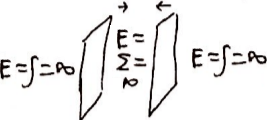
\includegraphics[width=0.32\textwidth]{./images/4-casimir}
		\caption{Casimir force between two parallel plates}
		\label{fig:casimir}
	\end{figure}
	\item The \emph{Lamb shift} is responsible of the breaking of the degeneracy between states $2 \, ^{2}s_{1/2}$ and $2 \, ^{2}p_{1/2}$ of hydrogen.
\end{itemize}

\subsubsection*{Spontaneous emission}
\begin{flalign*}
	\trn{E}^{2} &= -\sum_{j} \frac{\hbar \omega_{j}}{2 \varepsilon_{0} L^{3}} \qty(\cancel{\hat{a}_{j} \hat{a}_{j} e^{2i \va{k}_{j}\vdot\va{r}}} - \hat{a}_{j} \hat{a}_{j}\sdag - \cancel{\hat{a}_{j}\sdag \hat{a}_{j}} + \cancel{\hat{a}_{j}\sdag \hat{a}_{j}\sdag e^{-2i \va{k}_{j}\vdot\va{r}}} ) \Rightarrow \ev{\trn{E}^{2}}_{\ket{0}} = \sum_{j} \frac{\hbar \omega_{j}}{2 \varepsilon_{0} L^{3}} &
\end{flalign*}
But to recover the physical meaning, we need to do the limit when $L \to \infty$:
\begin{flalign*}
	\sum_{j} \frac{\hbar \omega_{j}}{2 \varepsilon_{0} L^{3}} &= \sum_{k_{j}} \sum_{\epsilon_{j}} \frac{\hbar c k_{j}}{2 \varepsilon_{0} L^{3}} \frac{(2\pi)^{3}}{(2\pi)^{3}} = \sum_{k_{j}} \frac{\hbar c k_{j}}{\varepsilon_{0} (2\pi)^{3}} \qty(\frac{2\pi}{L})^{3} & \\
	&\Rightarrow \int \frac{\hbar c k}{\varepsilon_{0} (2\pi)^{3}} \dd[3]{k} = \frac{\hbar c}{\varepsilon_{0} (2\pi)^{3}} \int k (k^{2} \dd{k} \dd{\Omega}) = \frac{\hbar c 4\pi}{\varepsilon_{0} (2\pi)^{3}} \int k^{3} \dd{k}
\end{flalign*}
Therefore,
\begin{align}
	(\Delta \trn{E}^{2})_{\ket{0}} = \ev{\trn{E}^{2}}{0} = \frac{\hbar c}{2 \varepsilon_{0} \pi^{2}} \int k^{3} \dd{k}
\end{align}
These fluctuations in the electric field are responsible of the spontaneous emission.

%-----------------------------------------------------------------
\subsection[Coherent states]{Coherent/quasi-classical states}
\begin{defi}[Coherent state, $\ket{\alpha}$]
	The coherent state is the eigenstate of the annihilation operator:
	\begin{subequations}
	\begin{align}
		\hat{a} \ket{\alpha} &= \alpha \ket{\alpha} \\
		\bra{\alpha} \hat{a}\sdag &= \alpha\sast \bra{\alpha} \\
		\comm*{\hat{a}}{\hat{a}\sdag} &\equiv \hat{\bbid}
	\end{align}
	\end{subequations}
\end{defi}
Coherent states are also called quasi-classical states because the expected values of the global and local operators correspond to the values of the classical fields:
\begin{align*}
	\left.
	\begin{aligned}
		\ev{\va{A}}{\alpha_{j}} &= \va{A}^{class}(\qty{\alpha_{j}}) \\
		\ev{\trn{H}}{\alpha_{j}} &= \trn{H}^{class}(\qty{\alpha_{j}}) \\
		\ev{\trn{\va{P}}}{\alpha_{j}} &= \trn{\va{P}}^{class}(\qty{\alpha_{j}}) \\
	\end{aligned}
	\right\}
	\Rightarrow
	\begin{aligned}
		\ev{\hat{a}_{j}}_{\alpha} &= \alpha_{j} \qc \forall j \\
		\ev{\hat{a}_{j}\sdag\hat{a}_{j}}_{\alpha} &= \alpha_{j}\sast \alpha_{j} \qc \forall j
	\end{aligned}
\end{align*}

\subsubsection*{Coherent states in the Fock basis}
A coherent state can be projected over the Fock basis: $\ket{\alpha} = \sum_{n=0}^{\infty} \ket{n} \braket{n}{\alpha}$. Let's work out the result of $\braket{n}{\alpha}$:
\begin{flalign*}
	\mel*{n-1}{\hat{a}}{\alpha} &= \sqrt{n} \braket{n}{\alpha} = \alpha \braket{n-1}{\alpha} = \alpha \bra{0} \frac{\hat{a}^{n-1}}{\sqrt{(n-1)!}} \ket{\alpha} = \frac{\alpha^{n}}{\sqrt{(n-1)!}} \braket{0}{\alpha} &\\
	\Rightarrow \braket{n}{\alpha} &= \frac{\alpha^{n}}{\sqrt{n!}} \braket{0}{\alpha} \Rightarrow \ket{\alpha} = \sum_{n=0}^{\infty} \frac{\alpha^{n}}{\sqrt{n!}} \braket{0}{\alpha} \ket{n}
\end{flalign*}
The value of $\braket{0}{\alpha}$ can be easily calculated considering that $\braket{a} \equiv 1$, and the fact that $\dsp \sum_{n=0}^{\infty} \frac{x^{n}}{n!} \equiv e^{x}$. Therefore, a coherent state in the Fock basis is
\begin{align}
	\ket{\alpha} = \sum_{n=0}^{\infty} \frac{\alpha^{n}}{\sqrt{n!}} e^{-\abs{\alpha}^{2}/2} \ket{n}
\end{align}

\subsubsection*{Particle aspects of a coherent state}
\begin{itemize}
	\item The photon number follows a Poisson distribution: $P(n) = \norm{\braket{n}{\alpha}}^{2} = e^{-\abs{\alpha}^{2}} \dfrac{\abs{\alpha}^{2n}}{n!}$.
	\item The expected value of the $\hat{N}$ and its variance are the same: $\ev*{\hat{N}} = (\Delta \hat{N})^{2} = \abs{\alpha}^{2}$.
	\item The relative variance vanishes in the classical limit: $\dfrac{\Delta \hat{N}}{\ev*{\hat{N}}} = \dfrac{1}{\abs{\alpha}} \underset{\abs{\alpha} \to \infty}{\longrightarrow} 0$.
\end{itemize}

\subsubsection*{Wave nature of a coherent state}
\begin{itemize}
	\item The expected value of $\trn{\va{E}}$ oscillates: $\ev{\trn{\va{E}}}{\alpha} = 2 \abs{\alpha} i \sqrt{\dfrac{\hbar \omega}{2 \varepsilon_{0} L^{3}}} \vu{\epsilon} \sin( \va{k} \vdot \va{r} - \omega t + \theta )$, where $\alpha = \abs{\alpha} e^{i \theta}$.
	\item The variance of $\trn{\va{E}}$ is independent of $\alpha$: $(\Delta \trn{\va{E}})^{2} = \dfrac{\hbar \omega}{2 \varepsilon_{0} L^{3}}$.
	\item The relative variance vanishes in the classical limit: $\dfrac{\Delta \trn{\va{E}}}{\ev*{\trn{\va{E}}}_{max}} = \dfrac{1}{2 \abs{\alpha}} \underset{\abs{\alpha} \to \infty}{\longrightarrow} 0$.
\end{itemize}

\subsubsection*{Scalar product and completeness}
\begin{itemize}
	\item $\dsp \braket{\alpha}{\beta} = e^{-\abs{\alpha}^{2}/2} e^{-\abs{\beta}^{2}/2} \sum_{n,m} \frac{\alpha\sast^{n}}{\sqrt{n!}} \frac{\beta^{m}}{\sqrt{m!}} \delta_{nm} = e^{-\abs{\alpha}^{2}/2} e^{-\abs{\beta}^{2}/2} e^{\alpha\sast \beta} = e^{-\abs{\alpha - \beta}^{2}/2}$, therefore, two different coherent states are not orthogonal.
	\item They form an over-complete set: $\dsp \frac{1}{\pi} \int \dyad{\alpha} \dd[2]{\alpha} = \bbid$, where $\alpha = \rho e^{i\theta}$ (figure \ref{fig:coherent-rep}).
\end{itemize}

\begin{figure}[H]
	\centering
	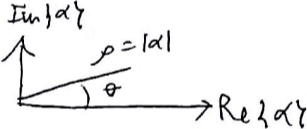
\includegraphics[width=0.3\textwidth]{./images/4-coherent-rep}
	\caption{Projection of a coherent state $\ket{\alpha}$ over the real and imaginary lines}
	\label{fig:coherent-rep}
\end{figure}

\subsubsection*{Coherent states are minimal states}
\begin{thm}[Heisenberg principle]
	If $\comm*{\hat{A}}{\hat{B}} = \hat{C}$, therefore $\Delta \hat{A} \cdot \Delta \hat{B} \geq \dfrac{1}{2}\ev*{\hat{C}}$.
\end{thm}

\begin{defi}[Quadratures of the electromagnetic field]
	The quadratures are hermitian operators that represent the real and imaginary parts of the complex amplitude represented by $\hat{a}$:
	\begin{align}
		\hat{X}_{1} = \hat{a}\sdag + \hat{a} \qc \hat{X}_{2} = i \qty(\hat{a}\sdag - \hat{a})
	\end{align}
	Therefore,
	\begin{align*}
		\underset{1\text{ mode}}{\trn{\va{E}}} = \mc{E}_{\omega} \vu{\epsilon} \qty{ \hat{X}_{1} \sin(\omega t - \va{k}\vdot\va{r}) - \hat{X}_{2} \cos(\omega t - \va{k}\vdot\va{r}) }
	\end{align*}
	The commutation relation between the two quadratures is
	\begin{align}
		\comm{\hat{X}_{1}}{\hat{X}_{2}} = 2i
	\end{align}
\end{defi}

\begin{itemize}
	\item The expected values of the quadratures are $\ev*{\hat{X}_{1}} = 2 \Re{\alpha}$, $\ev*{\hat{X}_{2}} = 2 \Im{\alpha}$.
	\item The uncertainties of the quadratures are $\Delta \hat{X}_{1,2} \equiv 1$. This is called the standard quantum limit.
\end{itemize}

Therefore, coherent states, $\ket{\alpha}$, are minimal states, meaning that they saturate the Heisenberg principle:
\begin{align}
	\Delta \hat{X}_{1} \Delta \hat{X}_{2} \equiv 1
\end{align}

\subsubsection*{Coherent states can be considered displaced vacuum}
\begin{thm}[Baker--Campbell--Hausdorff formula]
	If $\comm*{\hat{A}}{\comm*{\hat{A}}{\hat{B}}} = \comm*{\hat{B}}{\comm*{\hat{A}}{\hat{B}}} = 0$, therefore
	\begin{align}\label{eq:dumbledore}
		e^{\hat{A}+\hat{B}} = e^{\hat{A}} e^{\hat{B}} e^{-\comm*{\hat{A}}{\hat{B}}/2}
	\end{align}
\end{thm}
\begin{defi}[Displacement operator]
	The displacement operator is a unitary operator:
	\begin{align}
		\hat{\mc{D}}(\alpha) = \exp{\alpha \hat{a}\sdag + \alpha\sast \hat{a}}
	\end{align}
\end{defi}
\begin{subequations}
The displacement operator is not hermitian: $\hat{\mc{D}}\sdag(\alpha) \equiv \hat{\mc{D}}(-\alpha) = \hat{\mc{D}}^{-1}(\alpha)$. It can be shown that
\begin{align}
	\hat{\mc{D}}\sdag(\alpha) \hat{a} \hat{\mc{D}}(\alpha) &= \hat{a} + \alpha \\
	\hat{\mc{D}}\sdag(\alpha) \hat{a}\sdag \hat{\mc{D}}(\alpha) &= \hat{a}\sdag + \alpha\sast
\end{align}
\end{subequations}

Therefore, coherent states can be interpreted as displaced vacuum:
\begin{align}
	\ket{a} = \hat{\mc{D}}(\alpha) \ket{0}
\end{align}
Using the Baker--Campbell--Hausdorff formula \eqref{eq:dumbledore}, we can get $\ket{\alpha}$ in the Fock states basis.

\begin{itemize}
	\item Fock states are not minimal: $\braket{\hat{X}_{1,2}}{n} = 0$, $(\Delta \hat{X}_{1,2})^{2}_{\ket{n}} = 2n + 1$.
	\item But vacuum is: $(\Delta \hat{X}_{1,2})_{\ket{0}} \equiv 1$.
\end{itemize}

\begin{figure}[H]
	\centering
	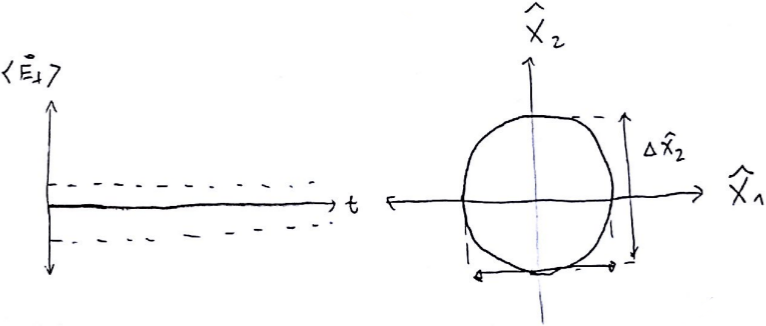
\includegraphics[width=0.7\textwidth]{./images/4-vacuum}
	% \caption{Representation of a the vacuum in the phase space}
	\caption{Representation of a the vacuum}
	\label{fig:vacuum}
\end{figure}
\begin{figure}[H]
	\centering
	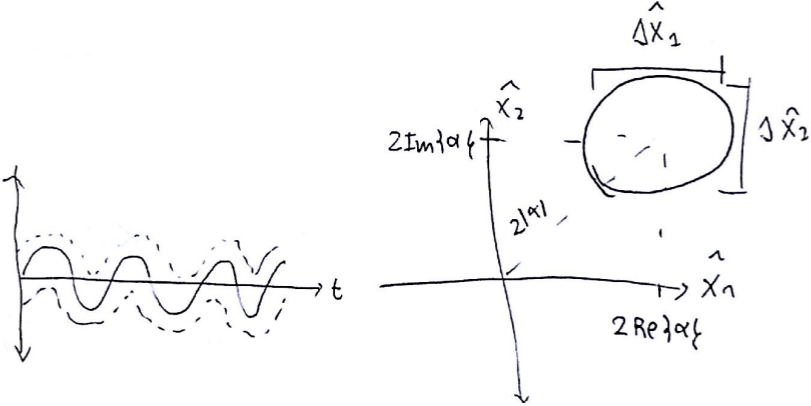
\includegraphics[width=0.75\textwidth]{./images/4-coherent}
	% \caption{Representation of a coherent state as displaced vacuum in the phase space}
	\caption{Representation of a coherent state as displaced vacuum}
	\label{fig:coherent}
\end{figure}

%-----------------------------------------------------------------
\subsection{Squeezed states}
\begin{defi}[Squeezed state, $\ket{s}$]
	A squeezed state is minimal ($\Delta \hat{X}_{1} \Delta \hat{X}_{2} \equiv 1$). Nonetheless, squeezed states break the standard quantum limit:
	\begin{align*}
		\begin{cases}
			\Delta \hat{X}_{1} < 1 \Leftrightarrow \Delta \hat{X}_{2} > 1 \\
			\Delta \hat{X}_{2} < 1 \Leftrightarrow \Delta \hat{X}_{1} > 1
		\end{cases}
	\end{align*}
\end{defi}
\begin{figure}[H]
	\centering
	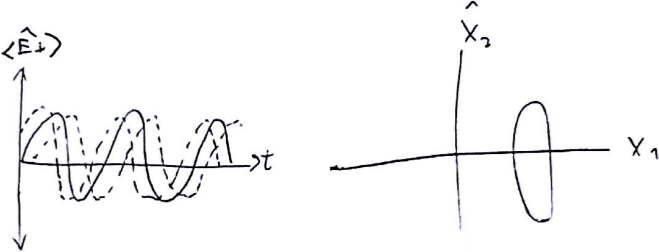
\includegraphics[width=0.7\textwidth]{./images/4-squeezed-x1}
	\caption{Representation of a squeezed state with $\Delta \hat{X}_{1} < 1$}
	\label{fig:squeezed1}
\end{figure}

\begin{figure}[H]
	\centering
	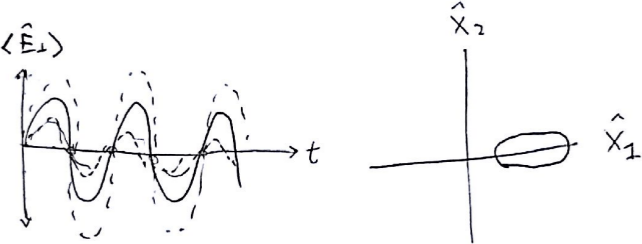
\includegraphics[width=0.7\textwidth]{./images/4-squeezed-x2}
	\caption{Representation of a squeezed state with $\Delta \hat{X}_{2} < 1$}
	\label{fig:squeezed2}
\end{figure}
\subsubsection*{Squeezing operator}
\begin{defi}[Squeezing operator]
	The squeezing operator is a unitary operator:
	\begin{align}
		\hat{\mc{S}}(z) = \exp{\frac{1}{2} \qty[z\sast \hat{a}^{2} - z \hat{a}\sdag^{2}]}
	\end{align}
	where $z = r e^{i \phi}$, $r$ being the squeezing parameter.
\end{defi}

\begin{subequations}
The squeezing operator is not hermitian: $\hat{\mc{S}}\sdag(z) \equiv \hat{\mc{S}}(-z) = \hat{\mc{S}}^{-1}(z)$. It can be shown that
\begin{align}
	\hat{\mc{S}}\sdag(z) \hat{a} \hat{\mc{S}}(z) &= \hat{a} \cosh r - \hat{a}\sdag e^{i\phi} \sinh r \\
	\hat{\mc{S}}\sdag(z) \hat{a}\sdag \hat{\mc{S}}(z) &= \hat{a}\sdag \cosh r - \hat{a} e^{-i\phi} \sinh r
\end{align}
\end{subequations}
Since squeezed states break the standard quantum limit, they can be interpreted as squeezed coherent states:
\begin{align}
	\ket{s} = \hat{\mc{S}}(z) \ket{\alpha}
\end{align}
For $\phi = 0$, $(\Delta \hat{X}_{1})^{2}_{\ket{s}} = e^{-2r} (\Delta \hat{X}_{1})^{2}_{\ket{\alpha}}$, and $(\Delta \hat{X}_{2})^{2}_{\ket{s}} = e^{2r} (\Delta \hat{X}_{2})^{2}_{\ket{\alpha}}$.

%-----------------------------------------------------------------
%	QUANTUM LIGHT-MATTER INTERACTION
%	!TEX root = ./../main.tex
%-----------------------------------------------------------------
\section{Quantum light--matter interaction}
\subsection{Jaynes--Cummings model}
Let's consider a two-level atom (figure \ref{fig:two-level-cummings}) and only one mode of the field.
\begin{figure}[H]
	\centering
	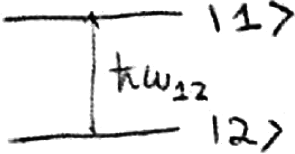
\includegraphics[width=0.2\textwidth]{./images/5-two-level-cummings}
	\caption{A two-level atom, where $\ket{2}$ is the ground state}
	\label{fig:two-level-cummings}
\end{figure}

In this system, an arbitrary state, $\ket{\psi}$ can be written as
\begin{align}
	\ket{\psi} = c_{1} \ket{1} + c_{2} \ket{2} = \mqty(c_{1} \\ c_{2})
\end{align}

\begin{defi}[Pauli matrices]
	\begin{align}
		\hat{\sigma}_{x} = \mqty(\pmat{1}) \qc \hat{\sigma}_{y} = \mqty(\pmat{2}) \qc \hat{\sigma}_{z} = \mqty(\pmat{3})
	\end{align}
\end{defi}

\begin{defi}[Lowering and rising operators]
	\begin{align}
		\hat{\sigma}_{+} = \frac{1}{2} (\hat{\sigma}_{x} + i \hat{\sigma}_{y}) = \mqty(0 & 1 \\ 0 & 0) \qc \hat{\sigma}_{-} = \frac{1}{2} (\hat{\sigma}_{x} - i \hat{\sigma}_{y}) = \mqty(0 & 0 \\ 1 & 0)
	\end{align}
	Therefore, in a two-level system, the lowering and rising operators act upon the atomic level:
	\begin{align*}
		\hat{\sigma}_{+} \ket{2} = \ket{1} \qc \hat{\sigma}_{-} \ket{1} = \ket{2}
	\end{align*}
\end{defi}

Let's work out the Hamiltonian, $\hat{H} = \hat{H}_{a} + \trn{\hat{H}} + \hat{V}$:
\begin{align}
	\hat{H}_{a} = \frac{\hbar}{2} \omega_{12} \hat{\sigma}_{z} \qc \trn{\hat{H}} = \hbar \omega \hat{a}\sdag \hat{a} \qc \hat{V} = - \hat{\va{\mu}} \vdot \trn{\hat{\va{E}}}
\end{align}
For the atomic Hamiltonian, $\hat{H}_{a}$, we've fixed the the origin of energy in the middle of $\ket{1}$ and $\ket{2}$. Now we need to develop the interaction Hamiltonian:
\begin{flalign*}
	\hat{V} &= - \hat{\va{\mu}} \vdot \trn{\hat{\va{E}}} = - \mu_{0} \trn{\hat{E}} (\hat{\sigma}_{-} + \hat{\sigma}_{+}) \overset{\text{EDA}}{\Longrightarrow} \trn{\hat{E}} = i \mc{E}_{\omega} (\hat{a} - \hat{a}\sdag) \Rightarrow \hat{V} = - i g \hbar (\hat{a} - \hat{a}\sdag) (\hat{\sigma}_{-} + \hat{\sigma}_{+}) & \\
	&= - ig \hbar (\underbrace{\hat{a} \hat{\sigma}_{-}}_{\text{(a)}} + \underbrace{\hat{a} \hat{\sigma}_{+}}_{\text{(b)}} - \underbrace{\hat{a}\sdag \hat{\sigma}_{-}}_{\text{(c)}} - \underbrace{\hat{a}\sdag \hat{\sigma}_{+}}_{\text{(d)}})
\end{flalign*}
\begin{figure}[H]
	\centering
	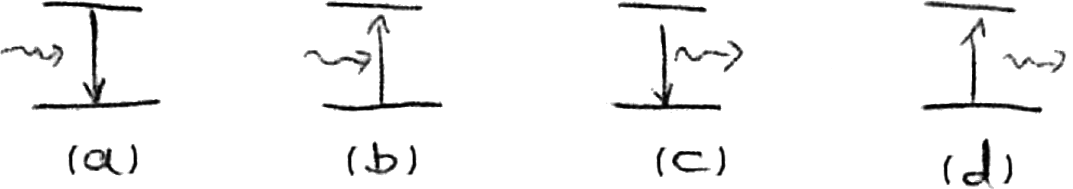
\includegraphics[width=0.6\textwidth]{./images/5-transitions}
	\caption{Possible atomic transitions: (b) is absorption, (c) is spontaneous emission, (a) and (d) are transitions that are only possible if they are fast enough}
	\label{fig:transitions}
\end{figure}
The pairs of operators have the following time dependence\footnote{We are considering the free evolution of the operators ($g = 0$).} in the Heisenberg picture:
\begin{subequations}
\begin{align}
	\hat{a}(t) \hat{\sigma}_{-}(t) &= \hat{a}(0) \hat{\sigma}_{-}(0) e^{-i(\omega + \omega_{0})t} \label{eq:asigma1} \\
	\hat{a}\sdag(t) \hat{\sigma}_{+}(t) &= \hat{a}\sdag(0) \hat{\sigma}_{+}(0) e^{i(\omega + \omega_{0})t} \label{eq:asigma2} \\
	\hat{a}(t) \hat{\sigma}_{+}(t) &= \hat{a}(0) \hat{\sigma}_{+}(0) e^{-i(\omega - \omega_{0})t} \label{eq:asigma3} \\
	\hat{a}\sdag(t) \hat{\sigma}_{-}(t) &= \hat{a}(\sdag0) \hat{\sigma}_{-}(0) e^{i(\omega - \omega_{0})t} \label{eq:asigma4}
\end{align}
\end{subequations}
The two first pairs (\ref{eq:asigma1},~\ref{eq:asigma2}) evolve at optical frequencies, which (near resonance) tend to average to zero in the course of a few optical periods compared to the pairs (\ref{eq:asigma3},~\ref{eq:asigma4}). This amounts to the same physics and mathematics that we used in discussing the RWA. Therefore, we get
\begin{align}
	\hat{V} = - ig \hbar (\hat{a} \hat{\sigma}_{+} - \hat{a}\sdag \hat{\sigma}_{-} )
\end{align}
where $g$ is the quantised Rabi frequency.

\begin{defi}[Quantised of the Rabi frequency]
	\begin{align}
		g \equiv \frac{\mu_{0} \mc{E}_{\omega}}{\hbar}
	\end{align}
\end{defi}

It's easy to prove in the Heisenberg picture that the full Hamiltonian in the Jaynes--Cunnings model is
\begin{align}
	\hat{H} = \underbrace{ \frac{\hbar}{2} \omega_{12} \hat{\sigma}_{z} + \hbar \omega \hat{a}\sdag \hat{a} }_{\hat{H}_{0}} - ig \hbar (\hat{a} \hat{\sigma}_{+} - \hat{a}\sdag \hat{\sigma}_{-} )
\end{align}

%-----------------------------------------------------------------
\subsection{Dressed atom}
\subsubsection*{Eigenstates}
The states $\ket{1, n}$ and $\ket{2, n}$ are eigenstates of the free Hamiltonian, $\hat{H}_{0}$, but the interaction Hamiltonian, $\hat{V}$, couples pairs of states (multiplets; $\xi_{n} = \qty{\ket{2, n+1}, \ket{1, n}}$) from the infinite set of eigenstates of the free Hamiltonian:
\begin{alignat*}{2}
	\hat{H}_{0} \ket{1, n} &= \qty(\frac{\hbar}{2} \omega_{12} + n \hbar \omega ) \ket{1, n} \qc & \hat{H}_{0} \ket{2, n+1} &= \qty(-\frac{\hbar}{2} \omega_{12} + (n+1) \hbar \omega ) \ket{2, n+1} \\
	\hat{V} \ket{1, n} &\mapsto \ket{2, n+1} \qc & \hat{V} \ket{2, n+1} &\mapsto \ket{1, n}
\end{alignat*}

Therefore, we can rewrite the full Hamiltonian as the sum of the Hamiltonians applied to each multiplet: $\hat{H} = \sum_{n} \hat{H}_{n}$, where the Hamiltonian applied to the multiplet $\xi_{n}$ is
\begin{align}
	\hat{H}_{n} = \hbar \qty(n + \frac{1}{2}) \omega \mqty(1 & 0 \\ 0 & 1) + \frac{\hbar}{2} \mqty( \Delta & - 2 i g \sqrt{n+1} \\ 2 i g \sqrt{n+1} & \Delta )
\end{align}
% WIP: Myestre says \mqty( \Delta & 2 g \sqrt{n+1} \\ 2 g \sqrt{n+1} & -\Delta )

\subsubsection*{Dressed states}
The dressed states of the two-level atom in the Jaynes--Cunnings model are
\begin{subequations}
\begin{align}
	\ket{-,n} &= \cos \theta_{n} \ket{1,n} - \sin \theta_{n} \ket{2,n+1} \\
	\ket{+,n} &= \sin \theta_{n} \ket{1,n} + \cos \theta_{n} \ket{2,n+1}
\end{align}
\end{subequations}
where $\Omega_{n}$ is the generalised quantised Rabi frequency, and $\theta_{n}$ are defined by
\begin{align*}
	\cos \theta_{n} = \frac{\Omega_{n} - \Delta}{\sqrt{(\Omega_{n} - \Delta)^{2} + 4 g^{2} (n+1)}} \qc \sin \theta_{n} = \frac{2 g \sqrt{n+1}}{\sqrt{(\Omega_{n} - \Delta)^{2} + 4 g^{2} (n+1)}}
\end{align*}

\begin{defi}[Generalised quantised Rabi frequency]
	\begin{align}
		\Omega_{n} \equiv \sqrt{\Delta^{2} + 4 g^{2} (n+1)}
	\end{align}
\end{defi}

The energies of the dressed states are
\begin{align}
	E_{n}^{\pm} = \hbar \qty(n + \frac{1}{2}) \omega \pm \frac{1}{2} \hbar \Omega_{n}
\end{align}

\begin{figure}[H]
	\centering
	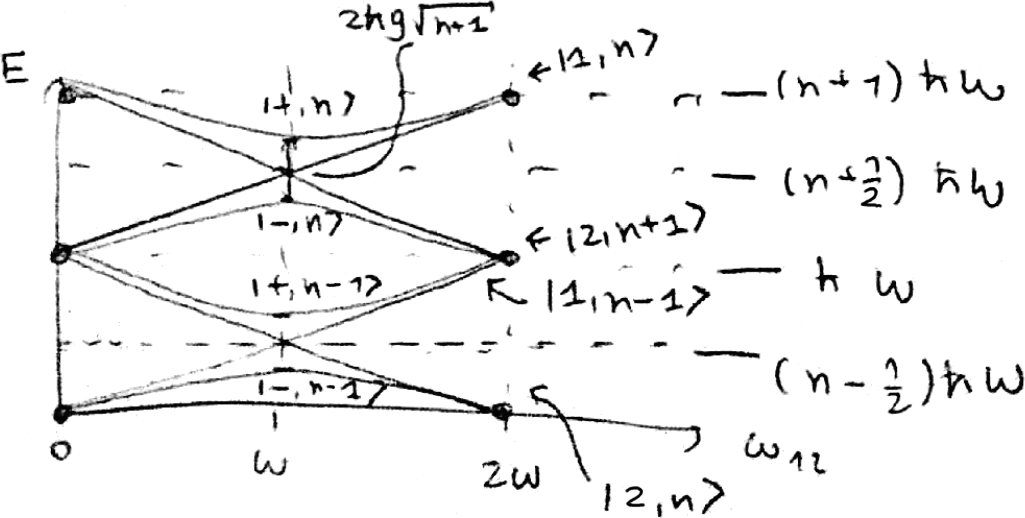
\includegraphics[width=0.7\textwidth]{./images/5-jc-energies}
	\caption{Energies of the dressed states under the Jaynes--Cunnings model}
	\label{fig:jc-energies}
\end{figure}

\subsubsection*{Mollow triplet}
In the Jaynes--Cunnings model, the photon emitted by spontaneous emission is not in the same mode of the Hamiltonian we are studying. Therefore, the atomic transition is between $\ket{1, n} \mapsto \ket{2, n}$. From the expressions of the dressed states we know that $\ket{1, n}$ is a linear combination of $\ket{+, n}$ and $\ket{-, n}$, whilst $\ket{2, n}$ is a linear combination of $\ket{+, n-1}$ and $\ket{-, n-1}$. Therefore, assuming that $\Omega_{n} \sim \Omega_{n+1}$ for a sufficiently large $n$, the transitions in the dressed basis are the following:
\begin{itemize}
	\item $\ket{-, n} \mapsto \ket{-, n-1} \Rightarrow E = \hbar \omega$.
	\item $\ket{-, n} \mapsto \ket{+, n-1} \Rightarrow E = \hbar (\omega - \Omega_{n})$.
	\item $\ket{+, n} \mapsto \ket{-, n-1} \Rightarrow E = \hbar (\omega + \Omega_{n})$.
	\item $\ket{+, n} \mapsto \ket{+, n-1} \Rightarrow E = \hbar \omega$.
\end{itemize}

\begin{figure}[H]
	\centering
	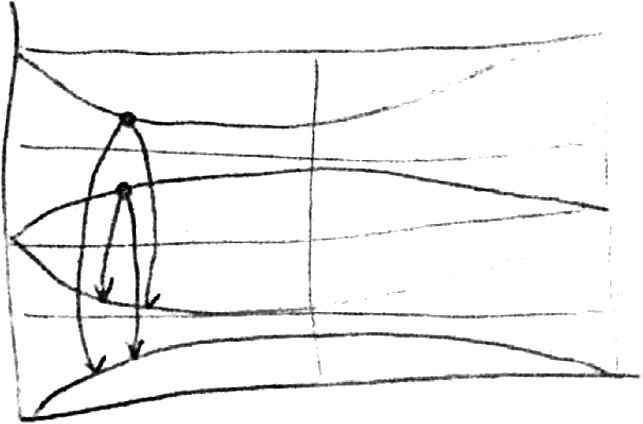
\includegraphics[width=0.5\textwidth]{./images/5-jc-mollow-triplet}
	\caption{Mollow triplet under the Jaynes--Cunnings model}
	\label{fig:jc-mollow-triplet}
\end{figure}

\subsubsection*{Autner--Townes doublet}
% WIP: expand from the exercises
\begin{figure}[H]
	\centering
	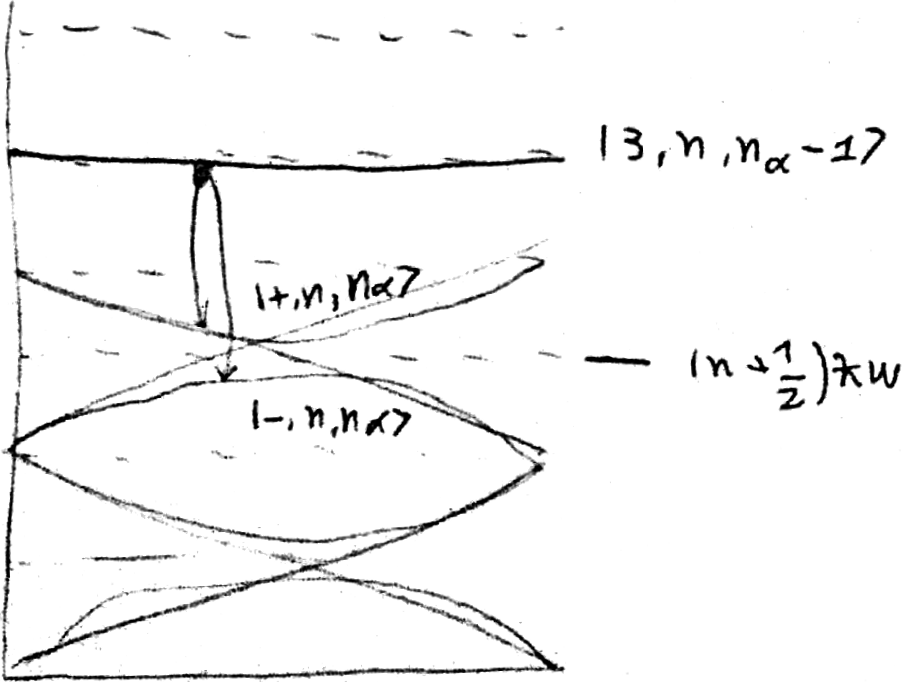
\includegraphics[width=0.55\textwidth]{./images/5-jc-autler-townes-doublet}
	\caption{Autner--Townes doublet under the Jaynes--Cunnings model}
	\label{fig:jc-autler-townes-doublet}
\end{figure}

%-----------------------------------------------------------------
\subsection{Quantum Rabi oscillations}
Since the dressed states, $\ket{\pm, n}$, are the eigenstates of the full Hamiltonian, we can use the integral form of the Schrödinger equation to calculate the temporal evolution of an arbitrary state, $\ket{\psi (t)}$:
\begin{flalign*}
	\ket{\psi(t)} &= \exp\qty{- i \frac{\hat{H}}{\hbar} t} \ket{\psi(0)} = \sum_{n=0}^{\infty} \sum_{j=\pm} \exp{-i \frac{E_{n}^{j}}{\hbar} t} \ket{j,n} \braket{j,n}{\psi(0)} & \\
	&\Rightarrow \mqty(c_{-,n}(t) \\ c_{+,n}(t)) = \mqty(\exp{i \frac{\Omega_{n}}{2} t} & 0 \\ 0 & \exp{-i \frac{\Omega_{n}}{2} t} ) \mqty(c_{-,n}(0) \\ c_{+,n}(0))
\end{flalign*}
The dressed basis can be interpreted as a transformation of the bare basis:
\begin{align}
	\mqty(c_{-,n}(t) \\ c_{+,n}(t)) = T \mqty(c_{1,n}(t) \\ c_{2,n+1}(t)) \qc T = \mqty( \cos \theta_{n} & - \sin \theta_{n} \\ \sin \theta_{n} & \cos \theta_{n})
\end{align}

Therefore, we can find the temporal evolution of the bare basis, which can be simplified further applying the RWA:
\begin{flalign*}
	\mqty(c_{1,n}(t) \\ c_{2,n+1}(t)) &= T^{-1} \mqty(\exp{i \frac{\Omega_{n}}{2} t} & 0 \\ 0 & \exp{-i \frac{\Omega_{n}}{2} t} ) T \mqty(c_{1,n}(0) \\ c_{2,n+1}(0)) & \\
	&= \mqty( \cos(\dfrac{\Omega_{n}}{2} t) - i \dfrac{\Delta}{\Omega_{n}} \sin(\dfrac{\Omega_{n}}{2} t) & - i \dfrac{2 g}{\Omega_{n}} \sqrt{n+1} \sin(\dfrac{\Omega_{n}}{2} t) \\ - i \dfrac{2 g}{\Omega_{n}} \sqrt{n+1} \sin(\dfrac{\Omega_{n}}{2} t) & \cos(\dfrac{\Omega_{n}}{2} t) + i \dfrac{\Delta}{\Omega_{n}} \sin(\dfrac{\Omega_{n}}{2} t) ) \mqty(c_{1,n}(0) \\ c_{2,n+1}(0))
\end{flalign*}

With the initial conditions $c_{1,n}(0) \equiv 1$ and $c_{2,n}(0) \equiv 0$, it's easy to see that
\begin{align}
	\mqty(c_{1,n}(t) \\ c_{2,n+1}(t)) = \mqty( \cos(\dfrac{\Omega_{n}}{2} t) - i \dfrac{\Delta}{\Omega_{n}} \sin(\dfrac{\Omega_{n}}{2} t) \\ - i \dfrac{2 g}{\Omega_{n}} \sqrt{n+1} \sin(\dfrac{\Omega_{n}}{2} t) )
\end{align}

\subsubsection*{Populations}
Since the expressions for $c_{1,n}(t)$ and $c_{2,n+1}(t)$ are relatively simple, we can calculate the temporal evolution of the populations:
\begin{subequations}
\begin{align}
	P_{1,n} (t) &= \norm{c_{1,n}(t)}^{2} = \cos[2](\frac{\Omega_{n}}{2} t) + \frac{\Delta^{2}}{\Omega_{n}^{2}} \sin[2](\frac{\Omega_{n}}{2} t) \\
	P_{2,n+1} (t) &= \norm{c_{2,n+1}(t)}^{2} = \frac{4 g^{2} (n+1)}{\Omega_{n}^{2}} \sin[2](\frac{\Omega_{n}}{2} t)
\end{align}
\end{subequations}

In resonance ($\Delta = 0$), these expressions are much simpler:
\begin{align}
	P_{1,n} (t) = \cos[2](g \sqrt{n+1} \, t) \qc P_{2,n+1} (t) = \sin[2](g \sqrt{n+1} \, t)
\end{align}

This $\Omega_{n}$ Rabi frequency is special, because it depends on $n+1$. This means the vacuum has Rabi oscillations as well.
%-----------------------------------------------------------------
\subsection{Collapses and revivals}
If we illuminate the atom with a coherent state, $\ket{\alpha}$, instead of a Fock state, $\ket{n}$, then the population becomes a superposition of oscillations: $P_{1, \alpha} = \sum_{n} P(n) \norm{c_{1,n}(t)}^{2}$. In resonance we have
\begin{align}
	P_{1,\alpha} = e^{-\abs{\alpha}^{2}} \sum_{n} \frac{\abs{\alpha}^{2n}}{n!} \cos[2](g \sqrt{n+1} \, t)
\end{align}

Since we have a superposition of oscillations, the population decays because of the dephasing (collapse). However, the superposition is a discrete sum, so after a certain time, the oscillations start to be in phase again (revival).
\begin{figure}[H]
	\centering
	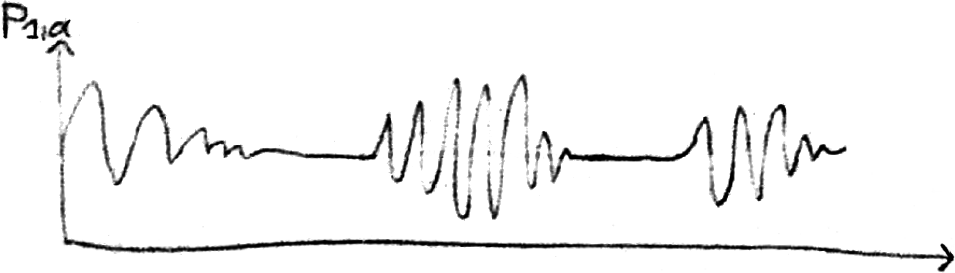
\includegraphics[width=0.7\textwidth]{./images/5-collapses-revivals}
	\caption{Collapses and revivals of the population}
	\label{fig:collapses-revivals}
\end{figure}
The collapse and revival times are given by
\begin{align}
	t_{c}(\Omega_{\ev{n} - \Delta n} - \Omega_{\ev{n} + \Delta n} ) \sim 1 \qc t_{r}(\Omega_{\ev{n}} - \Omega_{\ev{n} -1} ) \sim 2\pi m \qc m \in \mbb{N}
\end{align}

%-----------------------------------------------------------------
\subsection{Weisskopf--Wigner theory of spontaneous emission}
Armed with a proper three-dimensional density matrix formalism and the quantum light description, we can study the spontaneous emission of an excited state atom into the electromagnetic vacuum.
\begin{figure}[H]
	\centering
	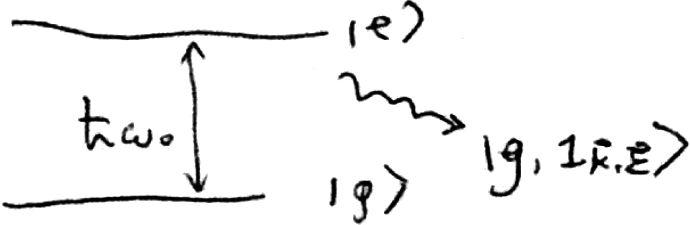
\includegraphics[width=0.4\textwidth]{./images/5-two-level-weisskopf}
	\caption{Spontaneous emission in a two level atom}
	\label{figtwo-level-weisskopf:}
\end{figure}

Let's work out the Hamiltonian, $\hat{H} = \hat{H}_{a} + \trn{\hat{H}} + \hat{V}$:
\begin{align}
	\hat{H}_{a} = \hbar \omega_{0} \dyad{e} \qc \trn{\hat{H}} = \sum_{\va{k},\vu{\epsilon}} \hbar \omega_{k} \qty(n_{\va{k},\vu{\epsilon}} + \frac{1}{2}) \qc \hat{V} = \sum_{\va{k},\vu{\epsilon}} \qty(\hbar g_{\va{k},\vu{\epsilon}} \hat{a}_{\va{k},\vu{\epsilon}} \hat{\sigma}_{+} + \Hc )
\end{align}
where $\hat{\mu} = \va{\mu}_{0} (\hat{\sigma}_{+} + \hat{\sigma}_{-})$, $\dsp \hat{E} = \sum_{\va{k},\vu{\epsilon}} i\qty(\mc{E}_{c} \vu{\epsilon}_{k} \hat{a}_{\va{k},\vu{\epsilon}} - \Hc )$, and $\dsp g_{\va{k},\vu{\epsilon}} = i \sqrt{\frac{\omega_{k}}{2 \hbar \varepsilon_{0} L^{3} }} \va{\mu}_{0} \vu{\epsilon}_{\va{k}}$.

Fixing the initial condition to $\ket{\psi (0)} = \ket{e, \qty{0}}$ reduces the general state vector to
\begin{align}
	\ket{\psi (t)} = c(t) e^{-i \omega_{0} t} \ket{e,\qty{0}} + \sum_{\va{k},\vu{\epsilon}} b_{\va{k},\vu{\epsilon}} (t) e^{-i \omega_{k} t} \ket{g, 1_{\va{k},\vu{\epsilon}}}
\end{align}
where $c(t)$ and $b_{\va{k},\vu{\epsilon}}(t)$ are, respectively, the probability amplitudes of the excited and ground states.

From the Schrödinger equation, $\dsp \hat{H} \ket{\psi (t)} = i \hbar \dv{\ket{\psi (t)}}{t}$, we can calculate the temporal evolution of the probability amplitudes:
\begin{subequations}
\begin{align}
	\dot{c}(t) &= i \sum_{\va{k},\vu{\epsilon}} g_{\va{k},\vu{\epsilon}} e^{-i (\omega_{k} - \omega_{0}) t} b_{\va{k},\vu{\epsilon}} (t) \\
	\dot{b}_{\va{k},\vu{\epsilon}}(t) &= i g_{\va{k},\vu{\epsilon}}\sast e^{i (\omega_{k} - \omega_{0}) t} c(t)
\end{align}
\end{subequations}
Let's work out the solution of $c(t)$:
\begin{flalign*}
	b_{\va{k},\vu{\epsilon}}(t) &= i g_{\va{k},\vu{\epsilon}}\sast \int_{0}^{t} e^{i (\omega_{k} - \omega_{0}) t'} c(t') \dd{t'} \Rightarrow \dot{c}(t) = - \sum_{\va{k},\vu{\epsilon}} \norm*{g_{\va{k},\vu{\epsilon}}}^{2} \int_{0}^{t} e^{-i(\omega_{k} - \omega_{0})(t - t')} c(t') \dd{t'} &
\end{flalign*}
Now we need to calculate the sum of $\norm*{g_{\va{k},\vu{\epsilon}}}^{2}$:
\begin{flalign*}
	\sum_{\va{k},\vu{\epsilon}} \norm*{g_{\va{k},\vu{\epsilon}}}^{2} &= \sum_{\va{k},\vu{\epsilon}} \frac{\omega_{k}}{2 \hbar \varepsilon_{0} L^{3}} (\va{\mu}_{0} \vdot \vu{\epsilon}_{\va{k}})^{2} \underset{L \to \infty}{\longrightarrow} \int \dd[3]{k} \sum_{\vu{\epsilon}} \frac{\omega_{k}}{2 \hbar \varepsilon_{0} (2 \pi)^{3}} (\va{\mu}_{0} \vdot \vu{\epsilon}(\va{k}))^{2} &\\
	&= \int_{0}^{\infty} \dd{k} k^{2} \frac{\omega_{k}}{2 \hbar \varepsilon_{0} (2 \pi)^{3}} \qty{ \sum_{j = 1}^{2} \int_{0}^{\pi} \sin \theta \dd{\theta} \int_{0}^{2\pi} \dd{\phi} (\va{\mu}_{0} \vdot \vu{\epsilon}_{j}(\va{k}))^{2} }
\end{flalign*}
Since $\qty{\vu{\epsilon}_{1}, \vu{\epsilon}_{2}, \va{k}}$ form an orthonormal basis, we can write any vector in that basis. In particular, we can write $\norm*{\va{\mu}_{0}}^{2} = (\va{\mu}_{0} \vdot \vu{\epsilon}_{1})^{2} + (\va{\mu}_{0} \vdot \vu{\epsilon}_{2})^{2} + (\va{\mu}_{0} \vdot \va{k})^{2}$. Geometrically, $(\va{\mu}_{0} \vdot \va{k})^{2} = \norm*{\va{\mu}_{0}}^{2} \cos^{2} \theta$; consequently, $\sum_{i = 1}^{2} (\va{\mu}_{0} \vdot \vu{\epsilon}_{i}(\va{k}))^{2} = \norm*{\va{\mu}_{0}}^{2} \sin^{2} \theta$. Therefore,
\begin{flalign*}
	\sum_{\va{k},\vu{\epsilon}} \norm*{g_{\va{k},\vu{\epsilon}}}^{2} &= \int_{0}^{\infty} \dd{k} k^{2} \frac{\omega_{k}}{2 \hbar \varepsilon_{0} (2 \pi)^{3}} \int_{0}^{\pi} \sin^{3} \theta \dd{\theta} \int_{0}^{2\pi} \dd{\phi} \norm*{\va{\mu}_{0}}^{2} = \frac{\norm*{\va{\mu}_{0}}^{2}}{6 \pi^{2} \varepsilon_{0} \hbar c^{3}} \int_{0}^{\infty} \omega_{k}^{3} \dd{\omega_{k}}. &
\end{flalign*}
Now that we have found an expression for $\sum_{\va{k},\vu{\epsilon}} \norm*{g_{\va{k},\vu{\epsilon}}}^{2}$, we can find a simpler expression for $\dot{c}(t)$. Since $\omega_{k} \sim \omega_{0}$, $e^{-i(\omega_{k} - \omega_{0})} \approx 1$, meaning that $\int \dd{\omega_{k}} e^{-i(\omega_{k} - \omega_{0})(t - t')} \approx 2 \pi \delta(t-t')$; this also means that the photon emitted by spontaneous emission will have the natural frequency of the two-level atom, $\omega_{0}$. Therfore,
\begin{flalign*}
	\dot{c}(t) &= - \frac{\norm*{\va{\mu}_{0}}^{2}}{6 \pi^{2} \varepsilon_{0} \hbar c^{3}} \int_{0}^{\infty} \omega_{k}^{3} \dd{\omega_{k}} \int_{0}^{t} e^{-i(\omega_{k} - \omega_{0})(t - t')} c(t') \dd{t'} & \\
	&\approx - \frac{\norm*{\va{\mu}_{0}}^{2}}{6 \pi^{2} \varepsilon_{0} \hbar c^{3}} \omega_{0}^{3} \int_{0}^{t} 2\pi \delta(t - t') c(t') \dd{t'} = - \frac{\norm*{\va{\mu}_{0}}^{2} \omega_{0}^{3}}{3 \pi \varepsilon_{0} \hbar c^{3}} c(t) \equiv - \Gamma c(t)
\end{flalign*}
Therefore, the temporal evolution of the probability amplitude of the excited state follows an exponential decay:
\begin{align}
	c(t) = e^{- \Gamma t} c(0) \qc \Gamma = \frac{\norm*{\va{\mu}_{0}}^{2} \omega_{0}^{3}}{3 \pi \varepsilon_{0} \hbar c^{3}}
\end{align}

Knowing the expression of $c(t)$, it's not difficult to see that, for $t \to \infty$, the probability amplitude of the ground state follows a Lorentzian:
\begin{align}
	\lim_{t \to \infty} \norm*{b_{\va{k}, \vu{\epsilon}}}^{2} = \frac{\norm*{g_{\va{k}, \vu{\epsilon}}}^{2}}{\Gamma^{2} + (\omega_{k} - \omega_{0})^{2}}
\end{align}

%-----------------------------------------------------------------
\subsection{Cavity quantum electrodynamics}
By using Rydberg atoms and a high-$Q$ cavity, one can realise the Jaynes--Cunnings model and treat the system as two-level atom and one mode of the electromagnetic field.

The reasons and advantages of using Rydberg atoms are:
\begin{itemize}
	\item Circular Rydberg atoms have a very large $n$ energy level (in Serge Haroche's experiments, $n \sim 50$).
	\item Only one electric dipole transition is allowed, which is very close to a two-level atom transition.
	\item They have very large classical radius ($r \sim n^{2} a_{0}$), therefore $\mu_{0} = \mel{n}{\mu}{n'} \sim e n^{2} a_{0}$.
	\item The decay rate is $\Gamma \propto \omega^{3}$. Since the transitions are in the microwave regime, the Rydberg atoms have a very long lifetime.
	\item They are easily ionisable, which is useful for the detection of the properties of the system.
\end{itemize}


%-----------------------------------------------------------------
%	BIBLIOGRAPHY
%-----------------------------------------------------------------
\nocite{b:steck}

\nocite{b:meystre}
\nocite{b:scully}
\nocite{b:walls}
\nocite{b:gerry}

\nocite{b:cohen-tannoudji-1}
\nocite{b:cohen-tannoudji-2}

% \printbibliography

\setcounter{secnumdepth}{0}
\section{Bibliography}
\printbibliography[title={Online}, keyword=web, heading=subbibliography]
\printbibliography[title={Basic}, keyword=basic, heading=subbibliography]
\printbibliography[title={Avanced}, keyword=advanced, heading=subbibliography]

%-----------------------------------------------------------------
\end{document}
